\documentclass[12pt,twoside]{article}
%
% declare a bold, tt font.
\DeclareFontShape{OT1}{cmtt}{bx}{n}{<5><6><7><8><9><10><10.95><12><14.4><17.28><20.74><24.88>cmttb10}{}
%
\usepackage[a4paper,margin=1in]{geometry}
\usepackage[OT1]{fontenc}
\usepackage{textcomp}
\renewcommand{\rmdefault}{ptm}
\usepackage[scaled=0.92]{helvet}
\usepackage{mtpro2}
\usepackage[sf,bf]{titlesec}
\usepackage[font=small,width=0.7\textwidth]{caption}
\usepackage{fancybox}
\usepackage{enumerate}
\usepackage{fancyhdr}
\usepackage{rotating}
\usepackage{picins,graphicx}
\usepackage[perpage,symbol]{footmisc}
\usepackage{tikz}
\usepackage{example}
\usepackage[super]{cite}
\usetikzlibrary{shapes,arrows,trees}
\usepackage[pdftex]{hyperref}
\newcommand{\samtrack}{\emph{SamTrack}}
\title{\sffamily\bfseries Crystallography Service \\ \samtrack\\ Administrator's Guide}
\author{J.P.Hagon\\Computer Systems Support\\School of Chemistry\\
Revision: Draft}
\date{\today}
\renewcommand{\abstractname}{Introduction}
%\renewcommand{\thefootnote}{\fnsymbol{footnote}}
%
\definecolor{skyblue}{rgb}{0.422,0.648,0.801}
\definecolor{darkgreen}{rgb}{0.0,0.4,0.0}
%
% Use these directives to change the appearance of example boxes.
%
\tikzstyle{plainbox} = [draw=blue, fill=skyblue!20, thin,
    rectangle, rounded corners, inner sep=5pt, inner ysep=5pt]
\tikzstyle{exmplbox} = [draw=blue, fill=skyblue!20, thin,
    rectangle, rounded corners, inner sep=5pt, inner ysep=15pt]
\tikzstyle{exmpltitle} =[draw=blue,fill=skyblue!50, text=white, thin]
%
% Headers
%
\pagestyle{fancy}
%
% define tikz block styles for flowcharts
%
\tikzstyle{decision} = [diamond, draw, fill=skyblue!20, 
    text width=7em, text badly centered, node distance=4cm, inner sep=0pt]
\tikzstyle{block} = [rectangle, draw, fill=skyblue!20, 
    text width=5em, text centered, rounded corners, minimum height=4em]
\tikzstyle{wideblock} = [rectangle, draw, fill=skyblue!20, 
    text width=10em, text centered, rounded corners, minimum height=4em]
\tikzstyle{line} = [draw, -latex']
\tikzstyle{cloud} = [draw, ellipse,fill=red!20, node distance=3cm,
    minimum height=2em]
%
\begin{document}
\maketitle
\begin{abstract}
This guide is intended for staff who administer the Newcastle University
Crystallography Service \samtrack\ Database.
It includes both a general description of the web interface and 
associated administration procedures along with a more technical
description of the software interface and the database itself so that
administrators can recover from situations such as a forgotten
administrator password.
\end{abstract}
\tableofcontents
\listoffigures
\listoftables
\newpage
\section{General Description of the System}
\subsection{Introduction}
\samtrack\ is a software application for tracking samples submitted to
the Newcastle University Crystallography Service.
The system consists of a \emph{front-end} which is used by users
and administrators to submit sample requests, upload analysis data,
edit sample status etc.  This front-end is implemented using the 
ruby\cite{rubybook,ruby} programming language and 
version 3 of \emph{Ruby on Rails}\cite{railsbook,rails}.
The front-end is hosted on an \emph{Apache}\cite{apache} server running on an
\emph{Ubuntu}\cite{ubuntu} linux system. 
Technical details will be described elsewhere.

The \emph{back-end} consists of a set of ruby programming libraries
and a SQL database --- in this case 
\emph{SQLite3}\cite{sqlite}.
More technical aspects of the back-end will be described elsewhere.

\subsection{Users}

The system has a relatively simple user setup with just one basic user
type. However, there are three levels of authority that a user can have:
\begin{description}
\item[Standard]
Most users of the system will have a standard account which allows them
to submit sample requests and view their own sample data.
\item[Group Leader]
These users have the additional privilege of being able to see all
of the sample data for their own group in addition to their own
samples. A group of users may have more than one designated group leader.
\item[Administrator]
An administrator, in addition to standard user privileges, can do many
administration tasks. These include adding/deleting users, changing user
privileges, submitting/updating/deleting samples, editing public web
pages on the server and uploading files to the server.
\end{description}

Users can either self-register or be added by an administrator.
An administrator can also disable a user account without actually
deleting it.
Only the most basic information about a user is stored in the database,
--- first name, last name and email address. the email address serves
as a login id. The user can set his own password. If the user forgets his
password, the system can email him a secure link to the server via which
the password can be reset.

\subsection{Groups}

All users must be associated with a group. Typically this will be a
research group associated with a particular person. When a user self-registers,
he must select an appropriate group. If such a group does not exist, an
administrator must set one up for him. Usually one or more users will be
designated \emph{group leaders} and will have access to information
about all the group's samples.

\subsection{Samples}

The primary purpose of the system is to track and keep a record of
samples submitted to the crystallography service. A typical work-flow is
shown in Figure \ref{fig:sample_workflow}.
Emails are sent automatically by the system when a sample status
is updated by an administrator.

\begin{figure}[!]
\small
\begin{center}
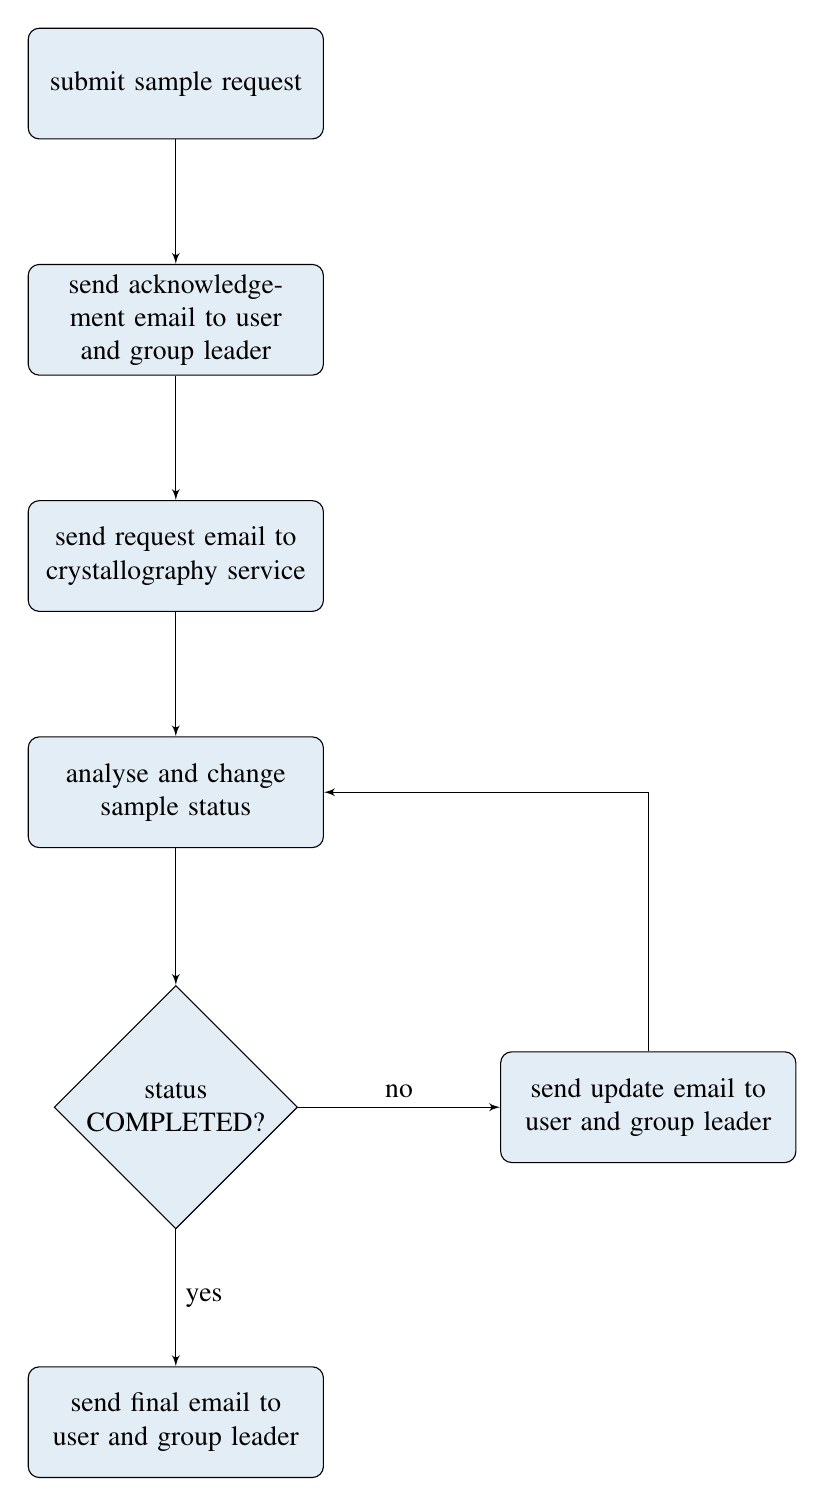
\begin{tikzpicture}[scale=2, node distance = 4cm, auto]
    % Place nodes
    \node [wideblock] (init) {submit sample request};
    \node [wideblock, below of=init, node distance=3cm] (email1) {send acknowledgement email to user
                                          and group leader};
    \node [wideblock, below of=email1, node distance=3cm] (email2) {send request email to
                                          crystallography service};
    \node [wideblock, below of=email2, node distance=3cm] (status) {analyse and change sample status};
    \node [decision, below of=status] (status1) {status\\COMPLETED?};
    \node [wideblock, right of=status1, node distance=6cm] (email4) {send update email to user
                                          and group leader};
    \node [wideblock, below of=status1] (email3) {send final email to user
                                              and group leader};
    % Draw edges
    \path [line] (init) -- (email1);
    \path [line] (email1) -- (email2);
    \path [line] (email2) -- (status);
    \path [line] (status) -- (status1);
    \path [line] (status1) -- node [, color=black] {no} (email4);
    \path [line] (status1) -- node [, color=black] {yes}(email3);
    \path [line] (email4) |- (status);
\end{tikzpicture}
\caption{Typical work-flow for sample processing cycle.
Emails are sent automatically by the system whenever the status of a
sample is updated.\label{fig:sample_workflow}}
\end{center}
\normalsize
\end{figure}

\subsection{The Sample Queue}
There are actually three queues defined in the system:
\begin{description}
\item[The Main Queue]
lists those samples which are awaiting initial analysis.
\item[The DLS Queue]
lists those samples which, after an initial analysis, were considered
to require further analysis at the \emph{Diamond Light Source} at
RAL.
\item[The Refinement (Ref) Queue]
lists those samples which have had initial analysis but require
further refinement.
\end{description}

\subsection{Public Pages}
Most information on the server can be viewed only by registered users.
However, there are some pages which are more generally accessible.
Such pages include the home page, general information pages and
the sample queue. Public pages can be created and edited by an administrator
using tools provided by the server software. rather than write pure
HTML, an administrator can use a text-based markup language called
\emph{Textile}\cite{textile}
which can produce sophisticated web pages with all the usual constructs
such as headings, paragraphs, floating elements, tables and images.

\section{Web Management Guide}
\subsection{Introduction}
In this section we describe the web management interface to the
sample tracking database. 
Before going through the basics of the web interface there is one
important point to make regarding the use of 
\emph{Microsoft Internet Explorer}:

\begin{plainblock}
There is a current issue with delete operations\footnote{This seems to affect
all Rails3 applications.} when using 
Internet Explorer. Basically, the delete operation will appear to work
but actually doesn't delete anything. All other operations which change the
database (create, edit) work fine but the delete operation does not.
For this reason, it is recommended that administrators use another browser
such as Firefox or Chrome when doing system management tasks.
\end{plainblock}

When a manager is logged-in, the home page of
the system looks similar to that shown in Figure \ref{fig:homepage}

\begin{figure}[!htb]
\begin{center}
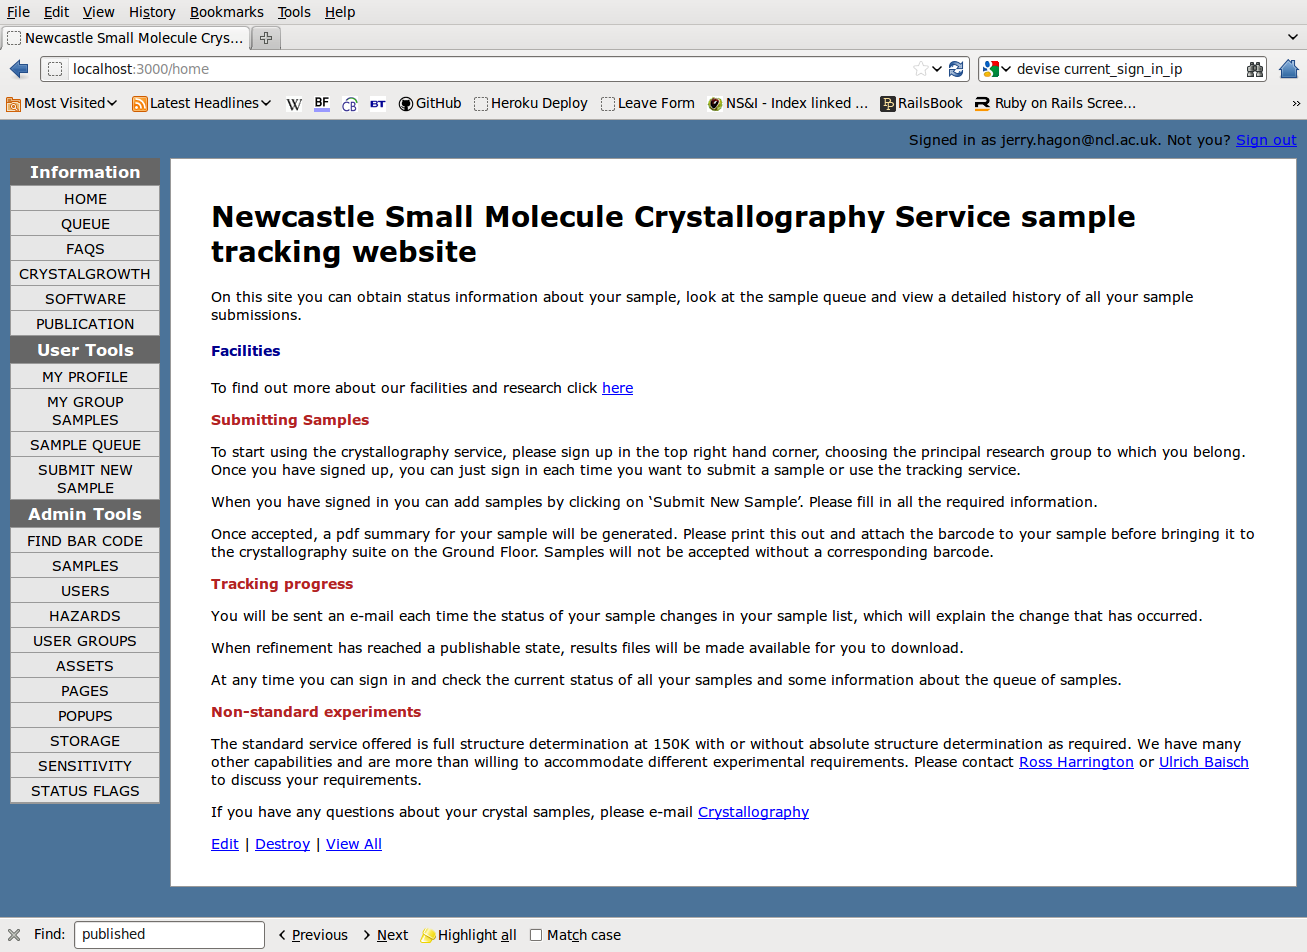
\includegraphics[width=0.65\textwidth]{homepage}
\caption{Administrator's view of home page.\label{fig:homepage}}
\end{center}
\end{figure}

There are three parts to this browser view:
\begin{enumerate}[(i)]
\item
a main display showing the contents of a page of information;
\item
a menu on the left side of the browser window;
\item
login information and a \verb=sign_out= link above the main display on
the right.
\end{enumerate}

The left side menu consists of three sections:
\begin{description}
\item[Information]
These links point to \emph{static} pages which can be created by an
administrator. the administrator can also add extra links to the
information section. We describe how to do this in \S\ref{sec:static}.
\item[User Tools]
These tools allow a user to view his sample list, submit a new sample
and view his profile information. Additionally, if a user is also a group
leader, he will have access to the \emph{My Group Samples} link for listing
all samples in the user's group.
\item[Admin Tools]
This is the main set of web-based tools for administrators. We will
describe each of these in the next section.
\end{description}
\subsection{Adding Static Pages}\label{sec:static}

\piccaption{The \emph{show}, \emph{edit} and \emph{delete} buttons.
\label{fig:showeditdelete}}
\parpic[r]{
\includegraphics{show}\quad
           
\includegraphics{edit}\quad
           
\includegraphics{delete}}
Clicking the \emph{PAGES} link in the \emph{Admin Tools} sub-menu 
produces the pages index shown in Figure \ref{fig:pageidx}.
This shows a list of pages. For each of these pages is a set of buttons
allowing the administrator to show, edit or delete the page as shown in
Figure \ref{fig:showeditdelete}.
These buttons are used throughout the database editing pages on the web server.
At the bottom of the list is a link to create a new page.

%\begin{figure}[!htb]
%\begin{center}
%
\includegraphics{show}\quad
%
\includegraphics{edit}\quad
%
\includegraphics{delete}
%\end{center}
%\caption{The \emph{show}, \emph{edit} and \emph{delete} buttons.
%\label{fig:showeditdelete}}
%\end{figure}

\begin{figure}[!htb]
\begin{center}
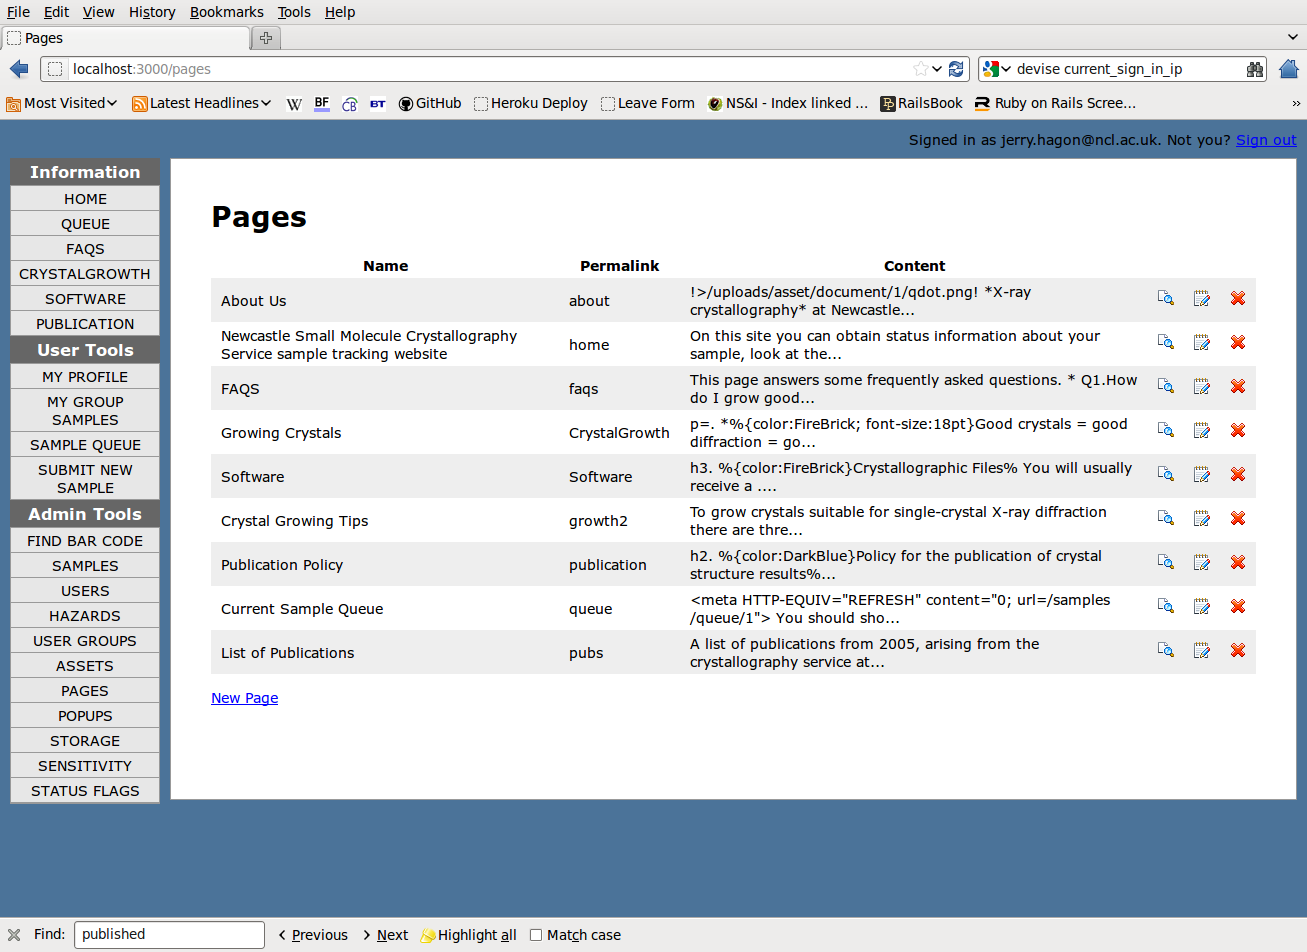
\includegraphics[width=0.65\textwidth]{pageidx}
\caption{The pages index view.\label{fig:pageidx}}
\end{center}
\end{figure}

\piccaption{The page edit view.\label{fig:editpage}}
\parpic[r]{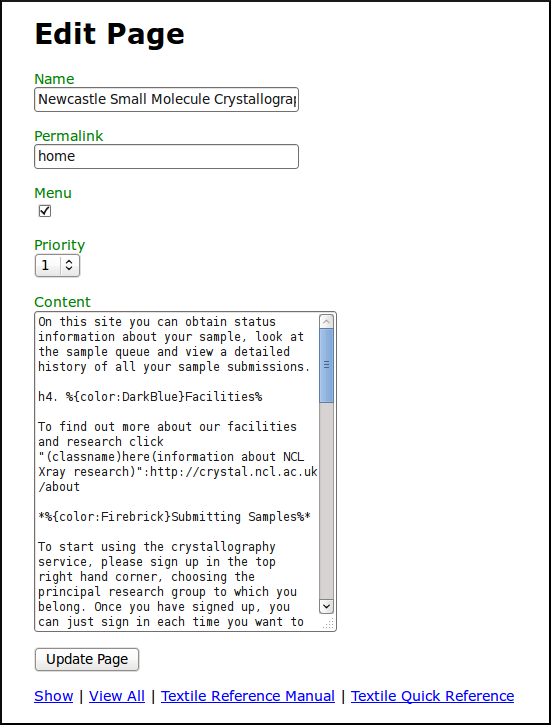
\includegraphics[width=0.4\textwidth]{editpage}}
Figure \ref{fig:editpage} shows the page editor --- a very simple form
for entering/changing text. This example shows the home page data. 
the content is entered in a markup language called Textile\footnote{You are 
allowed to mix HTML and Textile together.}. You can also specify the name
of the page (this will be used to set the HTML title attribute and a
permalink\footnote{A tag which is used as a basis for a concise URL.}.
At the bottom are links to the Textile Reference Manual, the page view
and the pages index. the page can be referred to via the URL:
\begin{verbatim}
<server name>/permalink
\end{verbatim}
thus making static page addressing very simple.
An alternative URL which can be generally used for any page is:
\begin{verbatim}
<server name>/pages/<id>
\end{verbatim}
but the permalink-based URL is what you'd almost always use in practice.
If, for some reason, you want to use the id-based URL, but don't know
what the id is, then just click the 'show' icon in the pages index for
the page you're interested in and look at the URL in the web browser window.

Note that there is also a checkbox labelled \emph{Menu}. If this is
checked then the page is added to the left hand \emph{Information} menu
of static pages. The \emph{Priority} parameter is an integer that
determines the order of the page in the menu. If two pages have the same
priority their order is determined alphabetically.
A good practice is to initially assign priorities in units of, say, 10.
Subsequently, if a new page is created, there are then plenty of 'spare'
priority numbers which can be used to add menu links in between
existing links --- otherwise existing priority numbers may need to be tweaked.

\subsection{Uploading General Files to the Server}
You can upload arbitrary files to the server. These files are referred
to as `assets' and can be uploaded via the \emph{ASSETS} link in the
\emph{Admin Tools} menu. Clicking on this link will take you to the
assets index page which looks very similar to the pages index described
in the previous section.
each index entry tells you the pathname of the file on the server,
together with a description of what the file contains. Often these files
will be images or documents (e.g. PDF files) that you want to link to
on one of the static web pages created as described in the previous
section.

At the bottom of the asset index list is a link to create a new asset.
Clicking this takes you to a simple menu where you can browse for a file
to upload to the server. Clicking the \emph{Create Asset} button will
then upload the file to the server. It will then be listed in the
asset index with an entry under the \emph{Document} column pointing
to its location in the file system. This location has the general form:
\begin{verbatim}
/uploads/asset/document/<id>/<filename>
\end{verbatim}
Here, \verb=<filename>= is the actual name of the uploaded file as it was
when it was uploaded. \verb=<id>= is the database id the document has
in the \verb=assets= table described in detail in \S\ref{sec:database}.
The actual URL of the document is then:
\begin{verbatim}
<servername>/uploads/asset/document/<id>/<filename>
\end{verbatim}

\subsection{Creating Users and Groups}
A user must belong to a group, so it is advisable to create a group for a
user before the user is created. Creating a user group is straightforward
via the \emph{USER GROUPS} link in the \emph{Admin Tools} menu.
As usual, this will take you to an index of existing groups, with a link
to create a new group at the bottom. Creating a new group merely requires
that you enter two fields:
\begin{enumerate}[(i)]
\item
a 3-letter group abbreviation (it \emph{must} be three letters);
\item
a longer group description.
\end{enumerate}

Users can be created in two ways; they can self-register by clicking
on the link top-right on the home page or they can be created by an
administrator. In either case the form used to create and register a new
user is the same.

\subsection{Sample Management}

In this section we give a complete description of the sample management
work-flow.
\begin{enumerate}[(i)]
\item
First, a user fills out a sample submission form online. This form is
shown in Figure \ref{fig:sampleform}. This figure shows the
submission form from the point of view of both a non-administrative user
and an administrator.
\begin{figure}[!htb]
\begin{center}
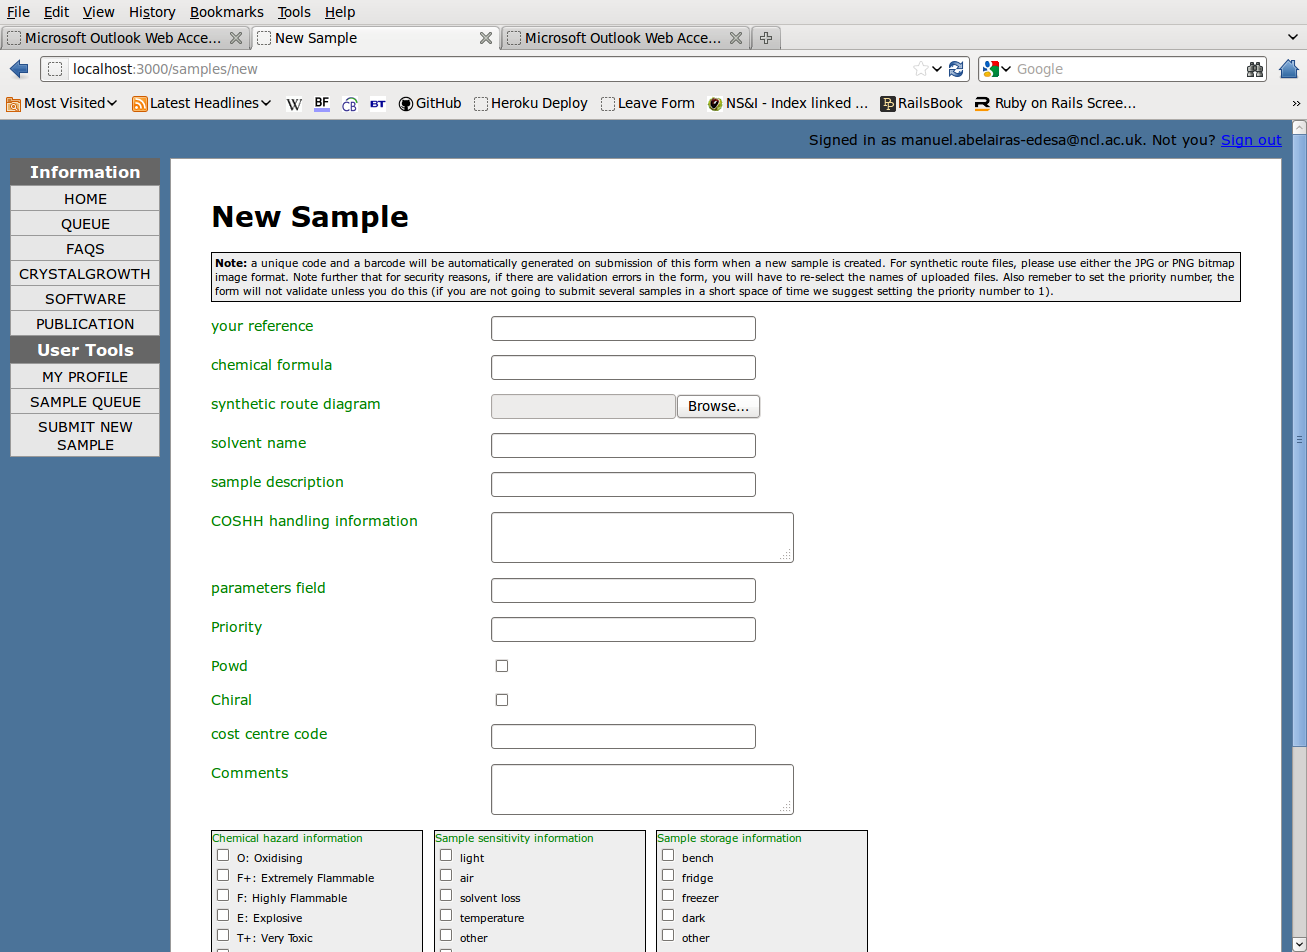
\includegraphics[width=0.45\textwidth]{sampleformuser}
\quad
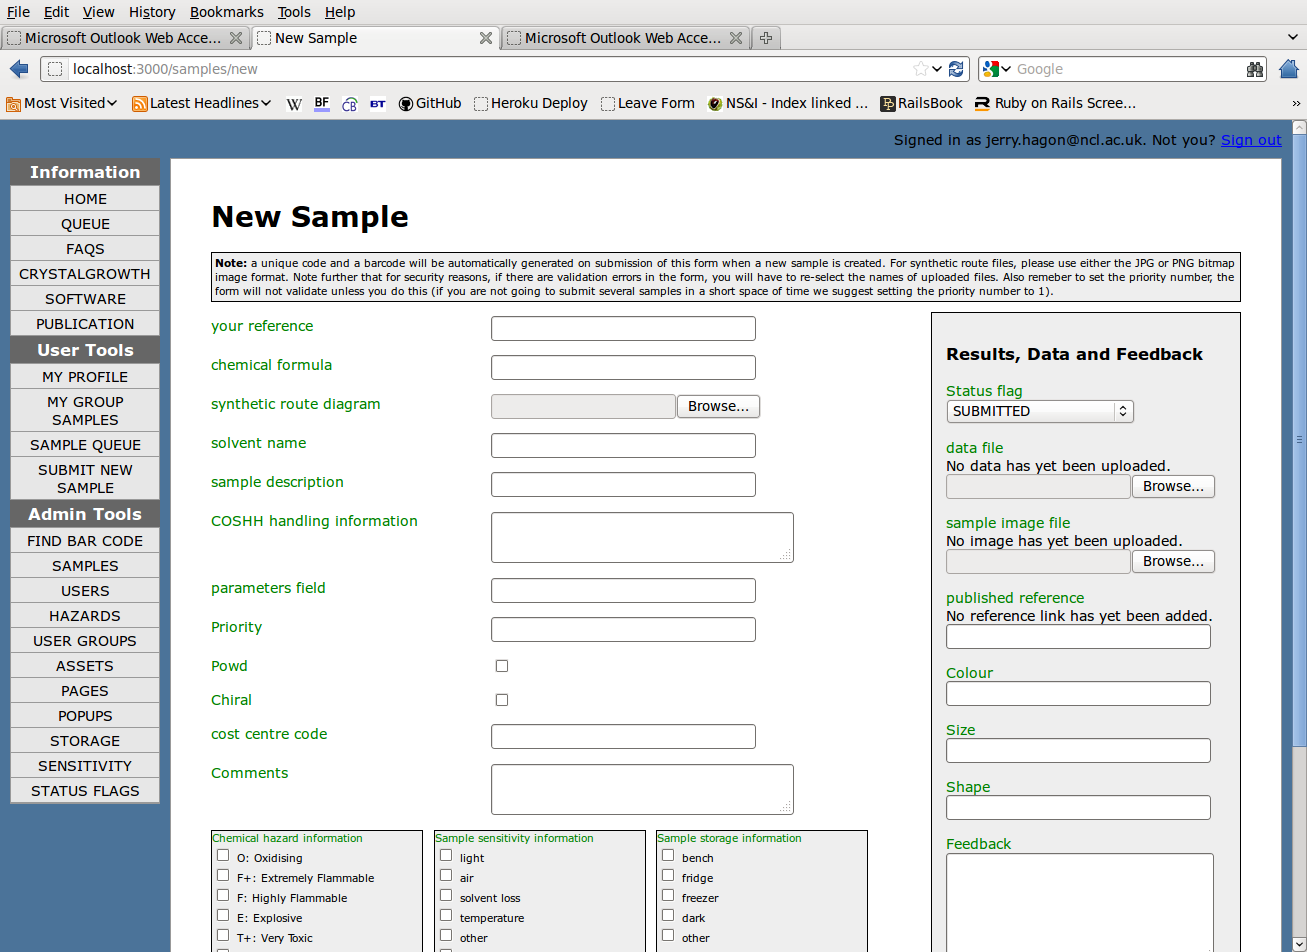
\includegraphics[width=0.45\textwidth]{sampleformadmin}
\caption{User's view (left) and administrator's view (right)
of the sample submission form.\label{fig:sampleform}}
\end{center}
\end{figure}

The bits that an ordinary user doesn't see are those parts of the sample
fields that are subsequently filled in by an administrator in the course
of sample processing.

There is a lot of validation built into the form making it very unlikely
that a form will be submitted with incomplete information.
Table \ref{tab:sampval} gives a complete list of
validation checks. If a validation check fails on submission of the form,
the user will be presented with the \emph{Invalid Fields} box which will
tell him which fields have not been entered correctly and what is
required. An extreme example of this is shown in Figure
\ref{fig:invalidfields} which shows what happens when none of the fields
in the form are filled-in.
\begin{table}{!htb}
\begin{center}
\begin{tabular}{lll}
\textbf{Field} & \textbf{Description} & \textbf{Validation} \\\hline
cif     &    chemical formula    &   can't be blank \\
synth   &    synthetic route diagram   &  must be supplied  \\
coshh\_name  &  name of solvent  &  can't be blank  \\
coshh\_info  &  COSHH handling information  &  can't be blank \\  
coshh\_desc  &  sample description  &  can't be blank  \\
params  &  unit cell parameters or CSD/Newcastle code  &  can't be blank \\ 
priority & user sample priority number & integer, range 1--9 \\
userref & user reference & alphanumeric without spaces \\
costcode & cost centre code & can't be blank
\end{tabular}
\caption{List of sample validation requirements.\label{tab:sampval}}
\end{center}
\end{table}

\begin{figure}[!htb]
\begin{center}
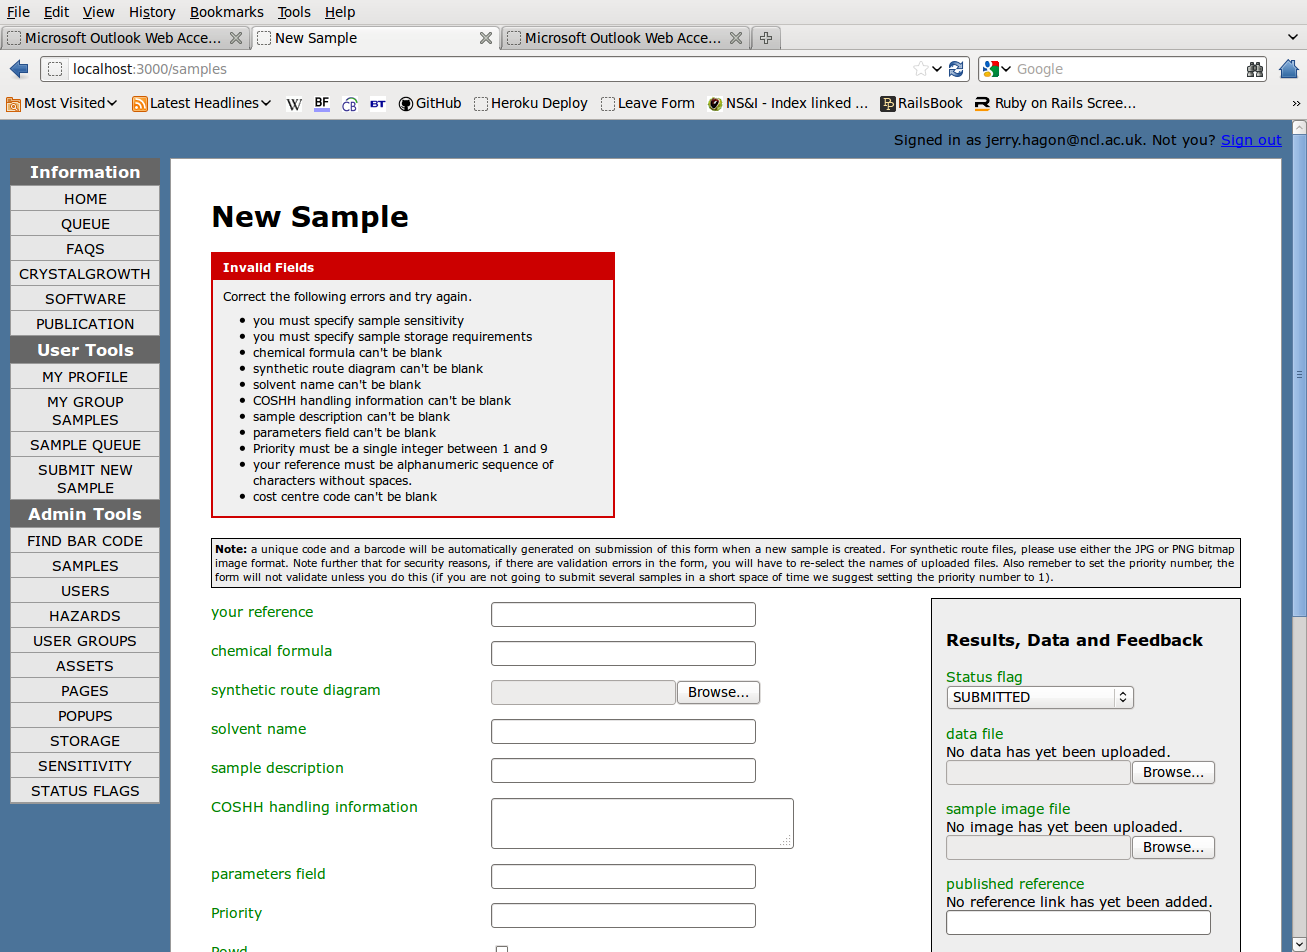
\includegraphics[width=0.45\textwidth]{invalidfields}
\quad
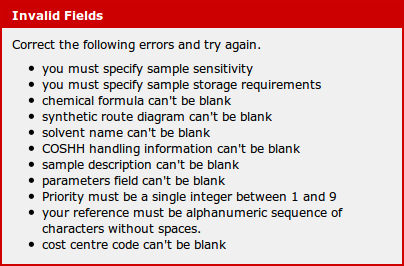
\includegraphics[width=0.45\textwidth]{invalidfieldsbox}
\caption{Illustrating what happens when an invalid form is submitted.
The user sees an \emph{Invalid Fields} box (shown enlarged on the right).
In this case, an administrative user has failed to fill in any of the fields
--- hopefully a very rare occurrence!\label{fig:invalidfields}}
\end{center}
\end{figure}

\item
On successful submission of the sample form, the user (and group leaders
if the user is not a group leader himself\footnote{If there is more than one
group leader then the other group leaders will also receive an email.}) 
will receive a confirmation email containing a link to the 
\emph{Sample Receipt} ---
a PDF file containing the user input information as well as a unique code
identifying the user, user group and sample and a unique bar code.
The email has the following general form with the tags in angle
brackets filled-in automatically:

\footnotesize
\begin{verbatim}
Dear User

New Sample Submission Code: <SAMPLE CODE> (your ref <SAMPLE USERREF>)
Submitted By: <USER FULL NAME>


your sample analysis request has been received. Please download a
receipt using the link below. Please quote the sample code in any
correspondence.

There is a tear-off slip at the bottom
of the receipt which you should attach to your sample.
You will be informed via email of any
changes in the status of your sample.

<LINK TO SAMPLE RECEIPT>

Copies of this email are sent to both sample submitters and their
research group leaders (where different).

Newcastle Crystallography Service
\end{verbatim}
\normalsize

A tear-off slip at the bottom of the sample receipt
containing the bar code, sample code and provided user
reference as well as essential COSHH information can be attached to the
actual sample itself.
Figure \ref{fig:samplereceipt} shows a typical sample receipt.

The receipt is generated on-the-fly from the supplied sample information. 
To perform the generation of the PDF, the well-known 
\href{http://prawn.majesticseacreature.com/}{Prawn} ruby library is used.
Once the sample has been submitted, a user can regenerate the sample receipt
at any time via a PDF link button in the sample list on his profile page
shown in Figure \ref{fig:userprofile}.

\begin{figure}[!htb]
\begin{center}
\fcolorbox{darkgreen}{white}{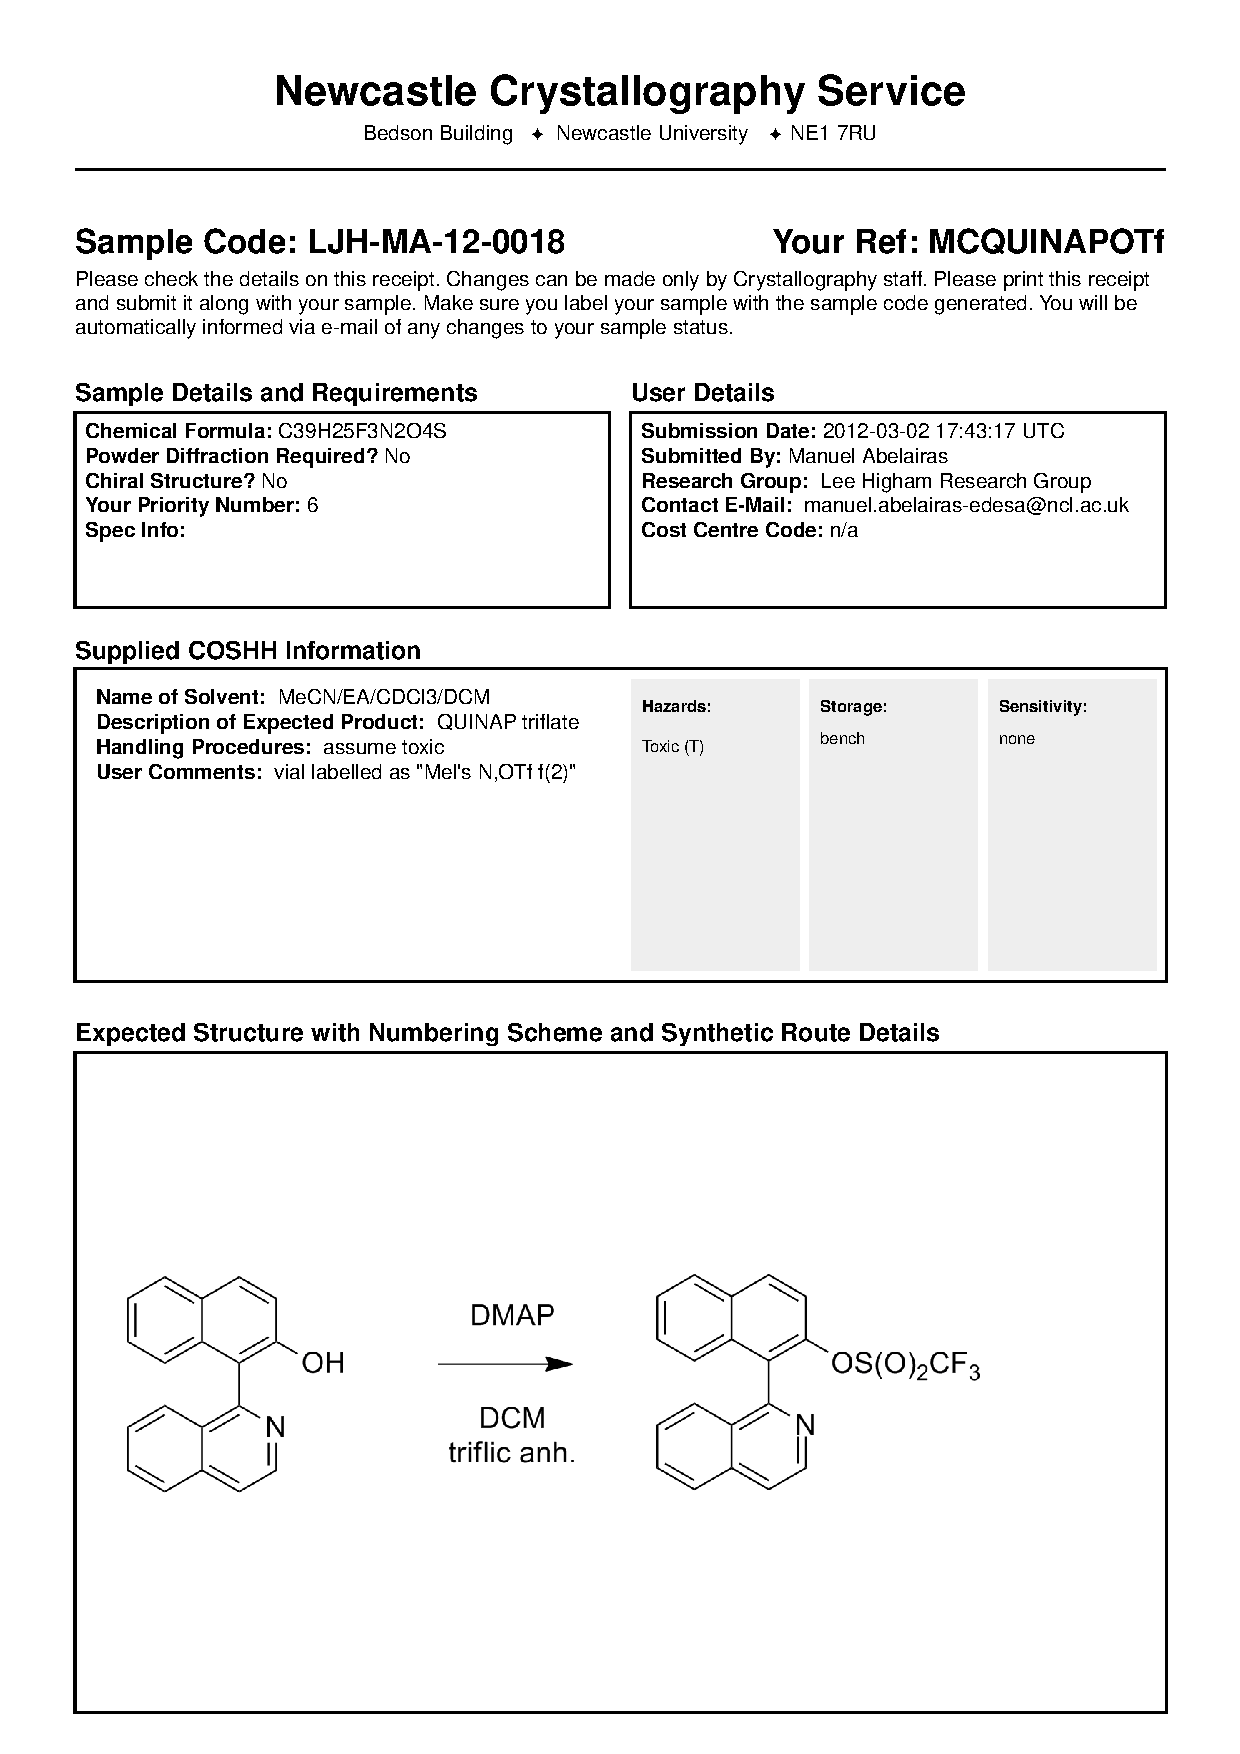
\includegraphics[width=0.9\textwidth]{samplereceipt}}
\caption{Example of a sample receipt (the actual size is A4).
Note the tear-off slip at the bottom. The receipt is generated
on-the-fly from the supplied sample information. The green border
is not part of the PDF rendering, it is used here merely to show
the A4 page border.\label{fig:samplereceipt}}
\end{center}
\end{figure}

\begin{figure}[!htb]
\begin{center}
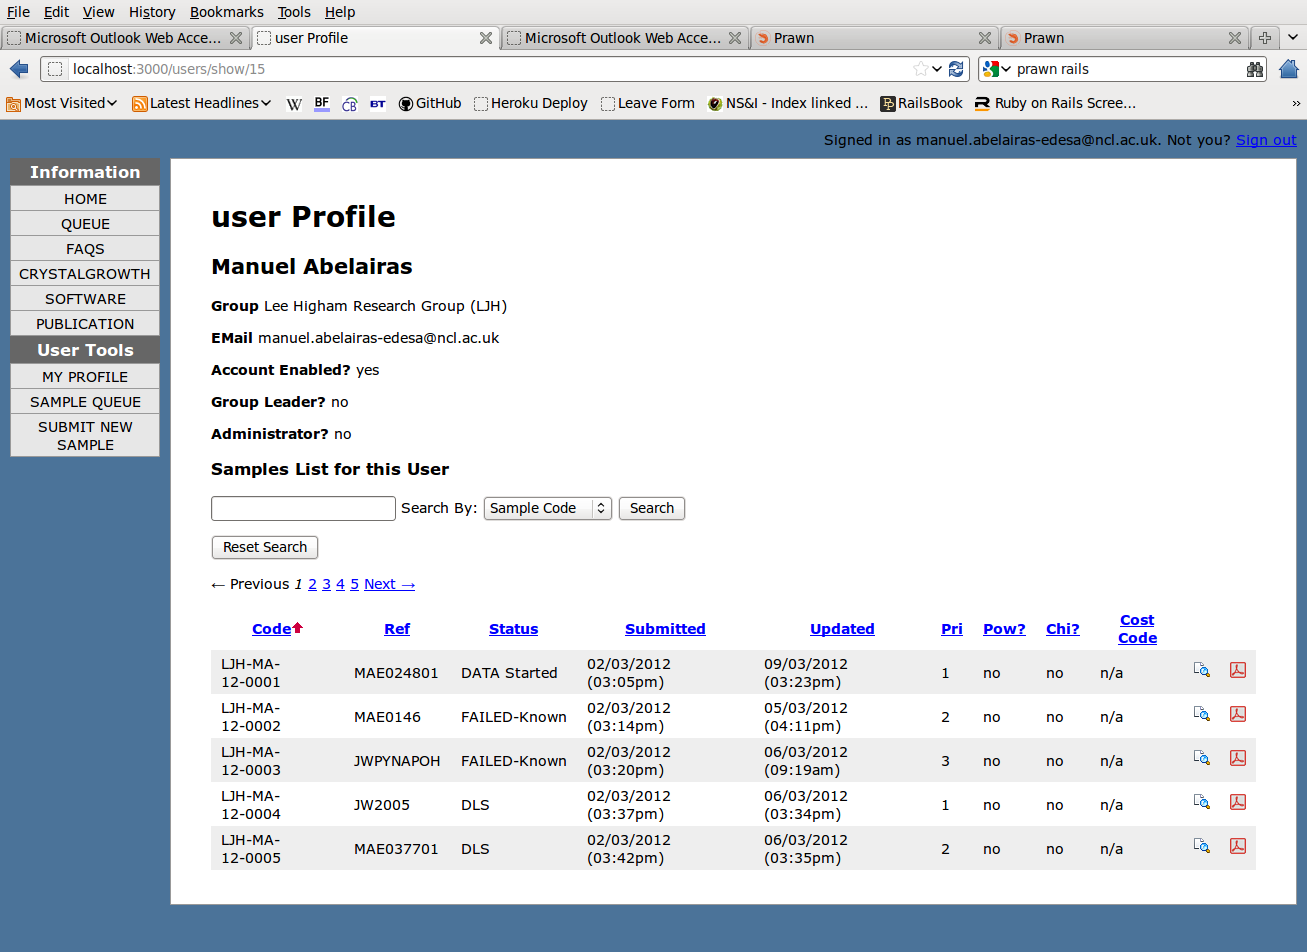
\includegraphics[width=0.65\textwidth]{userprofile}
\quad

\includegraphics{pdf.png}
\caption{User profile page showing sample list with PDF icon (shown
enlarged bottom right).\label{fig:userprofile}}
\end{center}
\end{figure}

\item
Next, the user brings his sample (with attached slip) for analysis and
at this point he should also see it in the sample queue.
\item
Initially the sample will have a status of \verb=SUBMITTED=. At various
points in the analysis, this status will be changed by crystallography
staff. Whenever the status is changed, an email is sent to both the user
and group leaders informing them of the change. The text of the email
looks similar to this:


\footnotesize
\begin{verbatim}
Dear User

This is to inform you that the status of sample
<SAMPLE CODE> (your ref <SAMPLE USERREF>) submitted by
<USER FULL NAME>
has changed as follows:

New Status: <NEW STATUS FLAG> <NEW STATUS FLAG DESCRIPTION>

Old Status: <OLD STATUS FLAG> <OLD STATUS FLAG DESCRIPTION>

<LINK TO FULL SAMPLE INFORMATION>

Copies of this email are sent to both sample submitters and their
research group leaders (where different).

Newcastle Crystallography Service
\end{verbatim}
\normalsize

\item
When crystallography staff have uploaded all results files (docx, res and
sample image) to the server and added any additional text feedback for
the sample, they will flag the sample as \verb=COMPLETED= and the process
will end. The sample data will continue to be available to users
(and administrators) indefinitely after that.

Results files (docx and res) will usually be made available in a single 
zip file, with
the sample image in a separate file. The files are uploaded by
administrators using the sample edit form shown in 
Figure \ref{fig:sampleeditform}. Note that only administrators have access
to the sample edit form.
Users will see the information in a slightly different way, not as a form
but as a standard 'show' page. This view is shown in
Figure \ref{fig:sampleeditform}.Note that if administrators do not fill in the feedback section, then a
default message `No feedback given.' is seen on the relevant part of the
sample show page. This is also illustrated in 
Figure \ref{fig:sampleshowpage}.

\begin{figure}[!htb]
\begin{center}
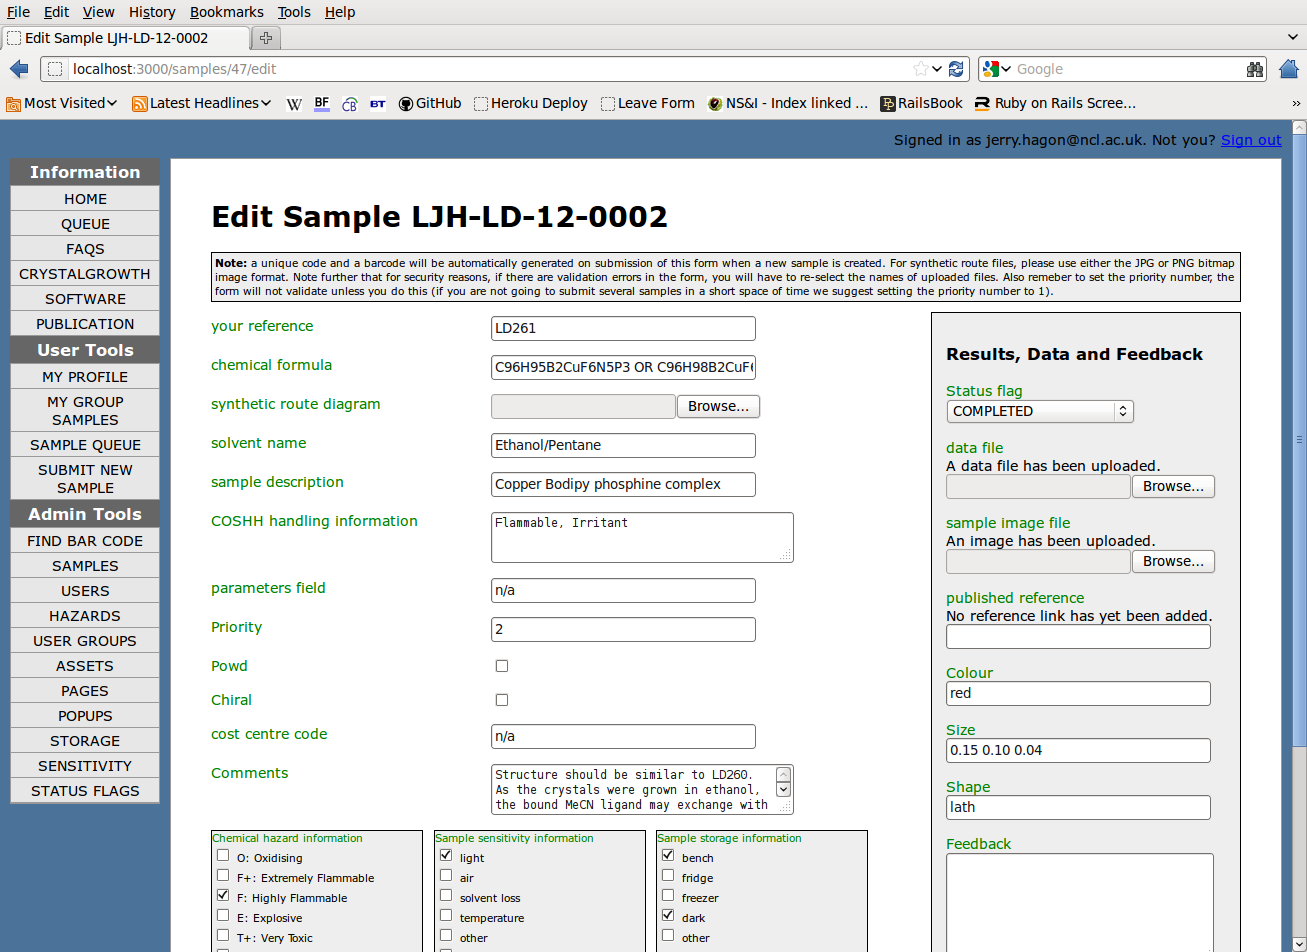
\includegraphics[width=0.75\textwidth]{sampleeditform}
\caption{A fully complete sample edit form.\label{fig:sampleeditform}}
\end{center}
\end{figure}

\begin{figure}[!htb]
\begin{center}
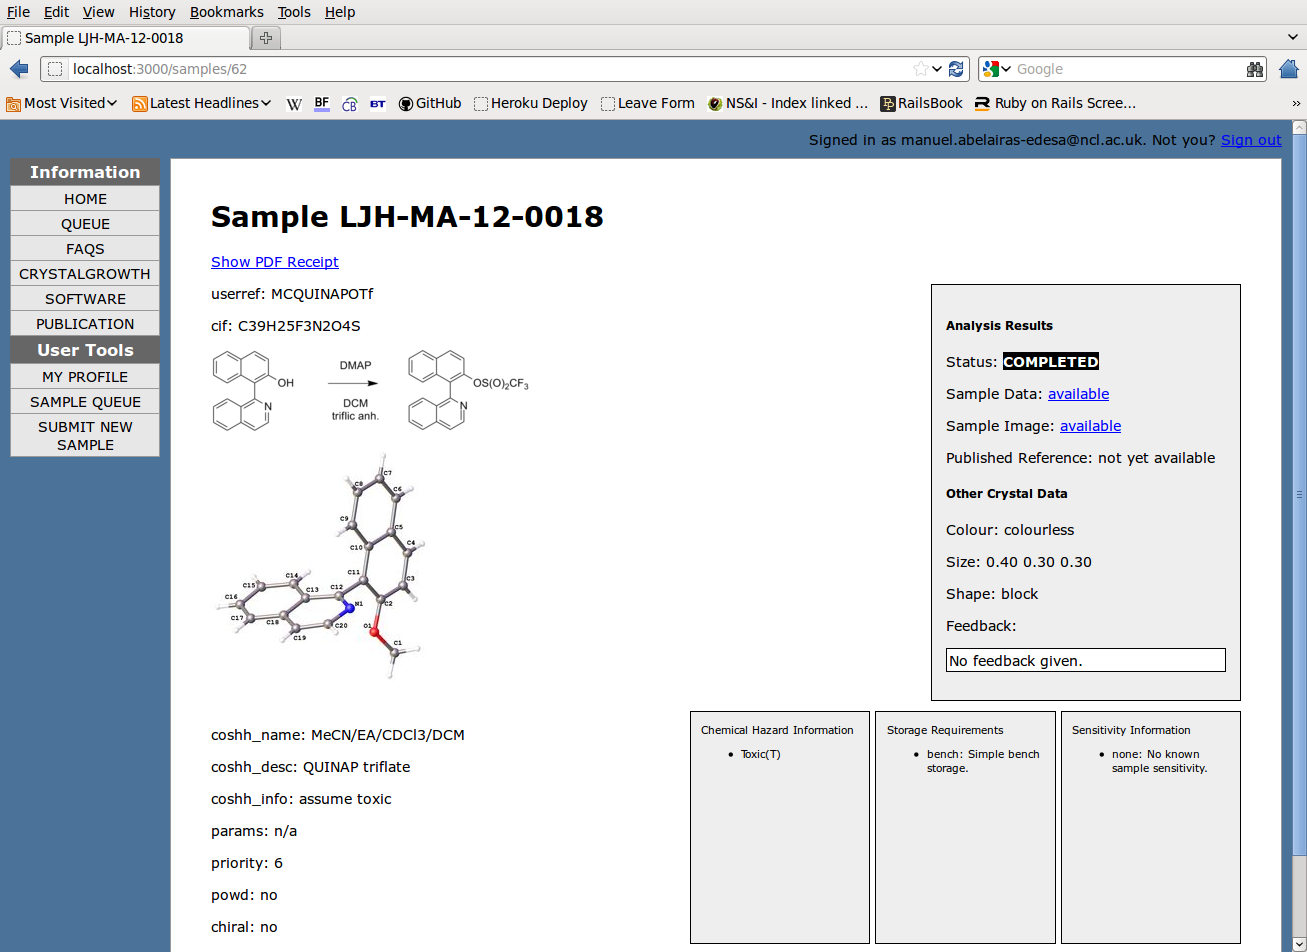
\includegraphics[width=0.60\textwidth]{sampleshowpage}
\quad
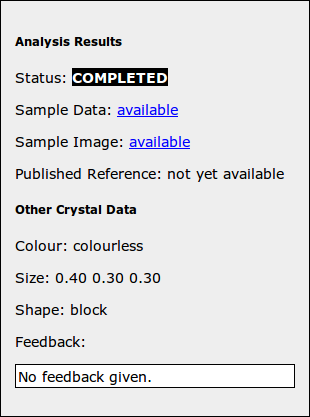
\includegraphics[width=0.30\textwidth]{sampleresults}
\caption{The user's view of a completed sample (left). On the right is
an enlarged view of the results section. Note also that a thumbnail image
of the sample is displayed. This thumbnail, when clicked, will show the
full-size image which can then be downloaded if desired.\label{fig:sampleshowpage}}
\end{center}
\end{figure}


\end{enumerate}

\subsection{Sample Search and Display Tools}
It is important that both administrators, group leaders and users can
find information about a particular sample or group of samples.
In this section we describe the tools that are available to quickly find
the sample data you need.

\begin{figure}[!htb]
\begin{center}
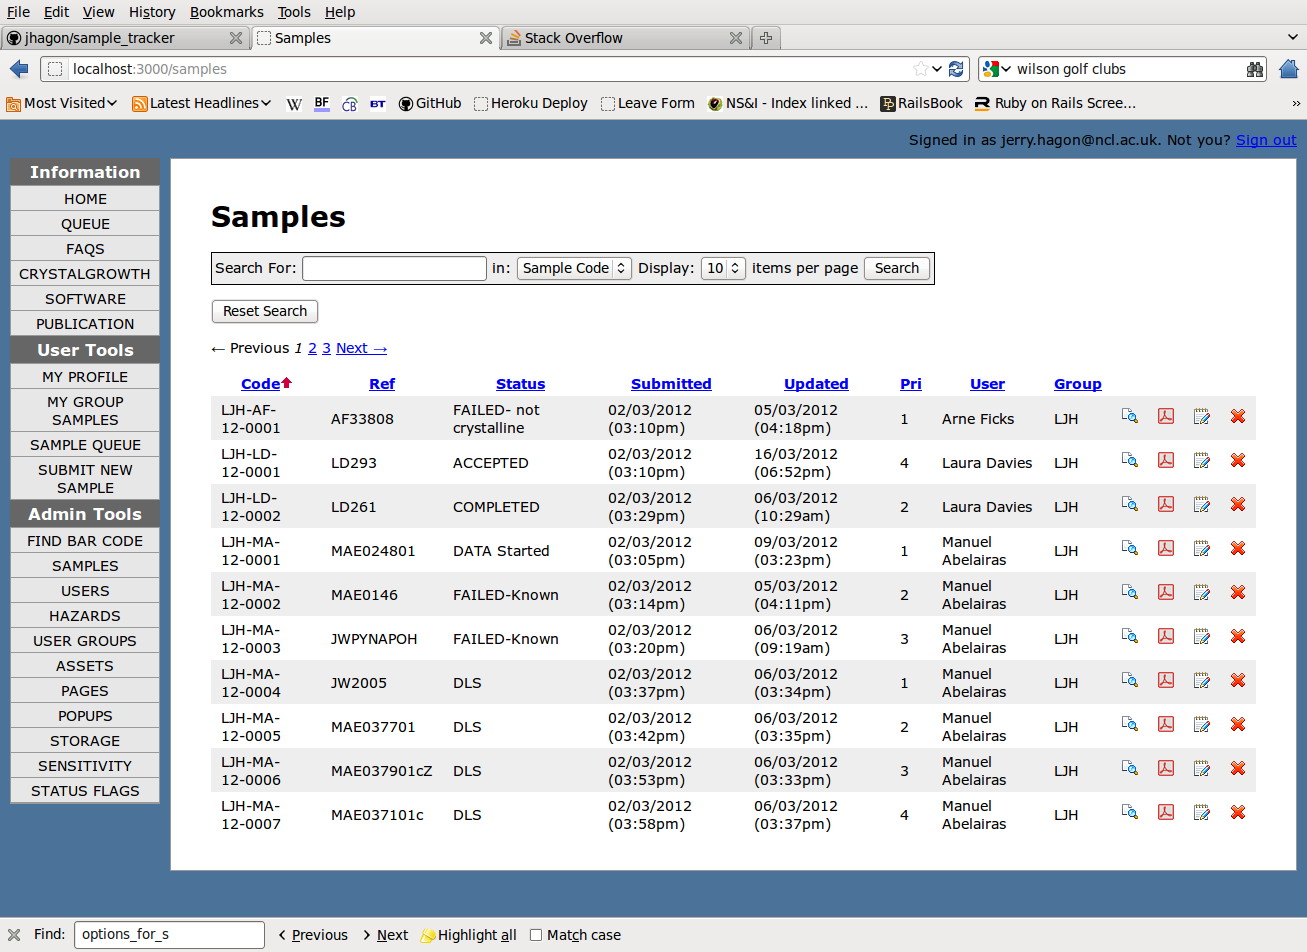
\includegraphics[width=0.75\textwidth]{sampleindex}
\caption{An administrator's view of the full sample index. 
In this case the red arrow next to the header in the \emph{Code}
column indicates that the list has been sorted by sample code in
ascending order (the default sorting).\label{fig:sampleindex}}
\end{center}
\end{figure}

For administrators, the usual starting point will be the main sample
index page shown in Figure \ref{fig:sampleindex}.
By default, this index is sorted by sample code in \emph{ascending} order.
This is indicated by a small red arrow pointing upwards next to the header
text in the \emph{Sample Code} column. 
Clicking the header text of the \emph{Sample Code} column will reverse the
order --- i.e. it will now be \emph{descending} order. This is indicated
by a blue arrow pointing downwards.
The list can be sorted on any other of the displayed columns simply by
clicking the column header. repeated clicking on the same column header
will toggle the sort order between ascending/descending.

The number of samples displayed per page can also be controlled by the
user. By default, this number is set by a global variable,
\verb=ITEMS_PER_PAGE= defined in the \verb=config/environment.rb= file\footnote{See the \emph{System Management} section for further details.}.
However, it can be easily changed by selecting the desired value from
a drop-down list in the search form above the sample list.
The first entry in this list is always the value in the
\verb=ITEMS_PER_PAGE= variable.
After the choice is made, the list will be re-paginated according to
the selected value. Note that for a full samples listing, the search box
itself must be empty when you do this.

\begin{figure}[!htb]
\begin{center}

\includegraphics[width=0.75\textwidth]{searchform}
\caption{The sample index search form. This is usually found
above the list of samples in most of the sample index pages.
\label{fig:searchform}}
\end{center}
\end{figure}

To narrow down the list of samples you need to type something into
the search box in the search form above the sample list. This search form
is common to most of the sample listing pages and is shown in
Figure \ref{fig:searchform}.
Currently You can search on three fields: 
the sample code, the user reference or the status. When you perform
a search, the results will be paginated according to the setting of the
pagination parameter described above. Note that search results can be
sorted as before by clicking the header text of the column that you
wish to sort by.
Below the search form is a reset button which resets all the search
parameters (but not the pagination) to their default values.

You can also use the standard SQL \verb=%= and \verb=_= symbols as `wildcard'
characters. The percent symbol maps to one or more characters in afield,
whereas the underscore maps to exactly one character.

For example if you want to search for all user references which contain
the letter sequence ABC followed by any set of characters followed
by 123, then you should enter ABC\%XYZ. The following strings would all
match this search:
\begin{verbatim}
ABC-XYZ  ABC123XYZ ABC1-2-3-XYZ ABCDXYZ
\end{verbatim}
However, only the first and last of the above strings would match if
ABC\_XYZ was entered instead. You can use any combination
of these wildcard characters in a string search.

\begin{plainblock}
Note that searches are \emph{not} cumulative --- they are always made
with respect to the full set of samples. In other words if you perform
a second search after an initial search, the results of the second search
will be exactly the same as if it had been performed first.
\end{plainblock}

\subsubsection{Bar Code Scanning}
\piccaption{A Zebex scanner.\label{fig:zebex}}
\parpic[r]{
\includegraphics[width=0.3\textwidth]{zebex}}
As mentioned earlier, each sample has associated with it a unique
bar code and it may sometimes be convenient to scan a sample bar code
and have the associated sample record displayed to the screen.
To this end, the system has a very simple interface which allows
a simple low-cost USB scanner such as the \emph{Zebex} scanner shown in 
Figure \ref{fig:zebex} to be used to extract a bar code.
The approach taken to facilitate this is brute force.

In the \emph{Admin Tools} menu is a link called \emph{Find Bar Code}.
Clicking this takes the user to a very simple form with just a single
entry field for a bar code. Now, assuming that the scanner is plugged in to
the same PC, if the mouse is clicked in the search box, then when the
scanner scans the bar code (usually a button needs to be pressed on the 
scanner) the actual code will magically appear in the box. Pressing
the search button on the form should then produce the matching sample
(see Figure \ref{fig:barcodeform}. 
For this to work correctly, the
bar code scanner needs to be put in \emph{keyboard emulation} mode.
Most scanners are capable of doing this, including the Zebex.
Of course, you can also type in the bar code by hand if you don't
have access to a scanner.

\begin{figure}[!htb]
\begin{center}
\fcolorbox{darkgreen}{white}{%
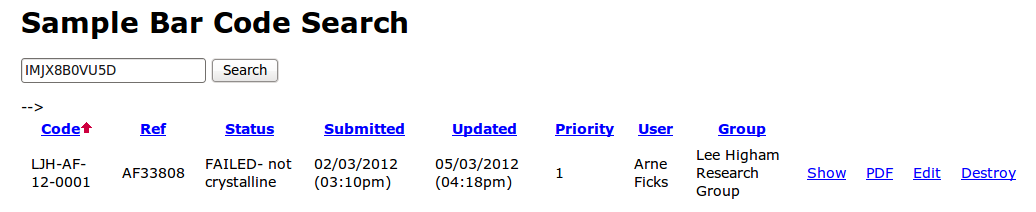
\includegraphics[width=0.75\textwidth]{barcodeform}}
\caption{A successful search using the \emph{Find Bar Code} form.
\label{fig:barcodeform}}
\end{center}
\end{figure}

\section{System Management and Internals}
\subsection{Introduction}
In this section we will explain lower-level aspects of the system
and its management.
This includes the operating system, command shell, web server, 
database, ruby language, ruby gems, and the rails3 system which is
used to do most of the programming.

\subsection{Basic Components of the System}
To begin with, we will describe the components of the system from the
operating system right up to the \emph{Rails3} software which is used
to write the web interface to the sample database.
Figure \ref{fig:systemcomponents} summarises the main components and
their relationships.

\begin{figure}[!htb]
\small
\begin{center}
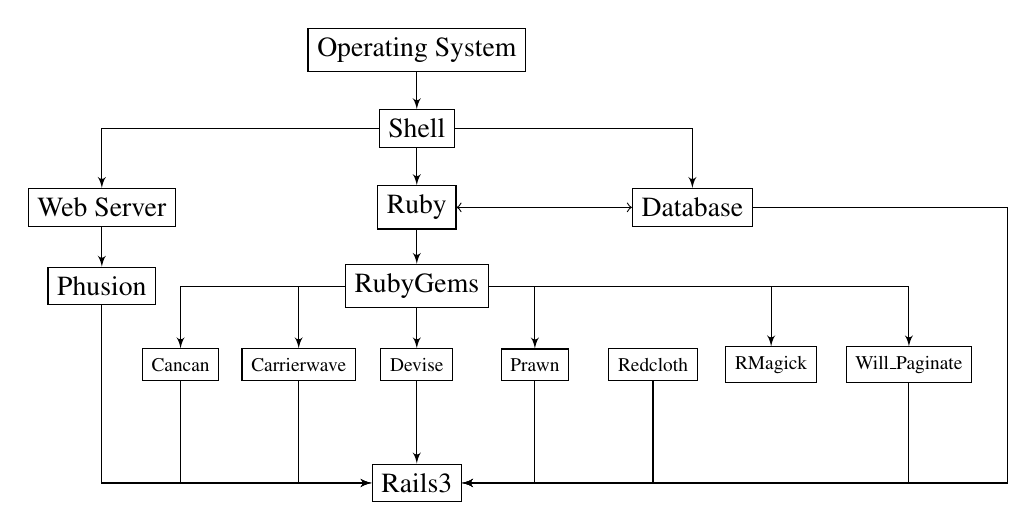
\begin{tikzpicture}
\node (os) at (0,1) [draw] {Operating System};
\node (shell) at (0,0) [draw] {Shell};
\node (web) at (-4,-1) [draw] {Web Server};
\node (database) at (3.5,-1) [draw] {Database};
\node (ruby) at (0,-1) [draw] {Ruby};
\node (phusion) at (-4,-2) [draw] {Phusion};
\node (gems) at (0,-2) [draw] {RubyGems};
\node (cancan) at (-3,-3) [draw] {\scriptsize Cancan};
\node (cwave) at (-1.5,-3) [draw] {\scriptsize Carrierwave};
\node (devise) at (0,-3) [draw] {\scriptsize Devise};
\node (prawn) at (1.5,-3) [draw] {\scriptsize Prawn};
\node (redcloth) at (3.0,-3) [draw] {\scriptsize Redcloth};
\node (rmagick) at (4.5,-3) [draw] {\scriptsize RMagick};
\node (willp) at (6.25,-3) [draw] {\scriptsize Will\_Paginate};
\node (rails) at (0,-4.5) [draw] {Rails3};
% draw lines
\path [line] (os) -- (shell);
\path [line] (shell) -| (web);
\path [line] (shell) -| (database);
\path [line] (shell) -- (ruby);
\path [line] (web) -- (phusion);
\path [line] (ruby) -- (gems);
\path [line,<->] (ruby) -- (database);
\path [line] (gems) -| (prawn);
\path [line] (gems) -| (cwave);
\path [line] (gems) -- (devise);
\path [line] (gems) -| (cancan);
\path [line] (gems) -| (rmagick);
\path [line] (gems) -| (willp);
\path [line] (phusion) |- (rails);

\path [line] (prawn) |- (rails);
\path [line] (cwave) |- (rails);
\path [line] (devise) -- (rails);
\path [line] (cancan) |- (rails);
\path [line] (willp) |- (rails);
\path [line] (redcloth) |- (rails);

\path [line] (database) -- (7.5,-1) |- (rails);
\end{tikzpicture}
\end{center}
\normalsize
\caption{The main components of the sample tracking system and their
relationships. This diagram takes a `top-down' view starting with
the operating system and moving through the various software layers
down to the rails3 system itself on which the sample tracking software
is based.\label{fig:systemcomponents}}
\end{figure}

Let's now look at each of these components individually:
\begin{description}
\item[Operating System]
The system runs on a computer running the Ubuntu version of the
linux operating system.
The specific release used at present is \emph{Ubuntu 10.04.3 LTS}.
Release 10.04 is also known via the code name `lucid'. LTS stands
for 'Long Term Support'. Extended support for this version will
last until 2014.
\item[Shell]
Access to most software on linux is vis a command shell. There are
many different shells available, the default being the \emph{bash}
shell. We will assume the use of bash throughout this guide, but
other shells can be also be used with little, if any modification
to the software itself.
\end{description}

Running under the shell are the three principal components of
the system: a web server, database and the ruby programming language
environment.
\begin{description}
\item[Web Server]
The web server we use is the ubiquitous \emph{Apache}, specifically
version 2.2.14.
\item[Ruby]
The version of ruby that comes with Ubuntu 10.04.3 is 1.8.7.
Unfortunately, this version is not recent enough to run a rails3
application. So, we use the \emph{Ruby Version Manager} to run a more
recent version of ruby (1.9.2).
\item[Database]
Rails 3 requires a database application to store and retrieve sample data.
We are using the \emph{SQLite3} database. This is a `lightweight' database
which requires very little separate maintenance. In particular, it
does not require a separate authentication process for access, nor
does it need to run a separate process in the background as with other
database software such as \emph{mysql}.
\end{description}

There are two other components of the system which sit between the
web server, ruby and database layer:

\begin{description}
\item[Phusion Passenger]
is an Apache module -- a `plugin' -- which
interfaces a rails3 application to the Apache web server. It also supplies
some debugging and error logging information which can be useful when
things go wrong.
\item[Ruby Gems]
are extension libraries to ruby. Some of them are
specific to rails3, but most have wider applicability and can be used in
more general applications. The ruby gems used in the sample tracking
application are described in the next section.
\end{description}

\subsubsection{Ruby Gems}
The following Ruby Gems are used in the application:
\begin{description}
\item[cancan\cite{cancan}]
written by well-known Rails programmer Ryan Bates is used for
authorisation. By this we mean controlling which parts of the application
can be accessed by users. For example, some parts of the application can
be accessed only by administrative users and others can be accessed by
anyone --- even those who have not registered to use the system.
\item[carrierwave\cite{carrierwave}]
is used to manage the upload of various files to the application
including data files, image files and general asset files.
\item[devise\cite{devise}]
is an authentication plugin to Rails which handles user data and
user authentication. It provides related functionality such as forgotten
password recovery (via email), user login statistics and more.
\item[prawn\cite{prawn}]
is a ruby library for producing PDF files. It is used to
auto-generate the sample receipts.
\item[redcloth\cite{redcloth}]
is a Ruby library used for parsing and display of Textile input.
\item[rmagick\cite{rmagick}]
is a well-known software application consisting of both
libraries and utility programs for manipulation of bitmap graphic files.
This gem interfaces the ImageMagick libraries to Ruby allowing
ImageMagick routines to be called from within a Ruby program.
\item[will\_paginate\cite{willp}]
is used to set up pagination of sample listings (and other things).
\end{description}

\subsection{Files and Directories}
In this section we describe the overall file and directory structure
of the application. Some of the files contain parameters which can be
changed to affect the behaviour of the application or the appearance
of the views. The overall directory structure is shown in
Figure \ref{fig:filestructure}.

\begin{sidewaysfigure}
\captionsetup{width=20cm}
\begin{center}
\scriptsize
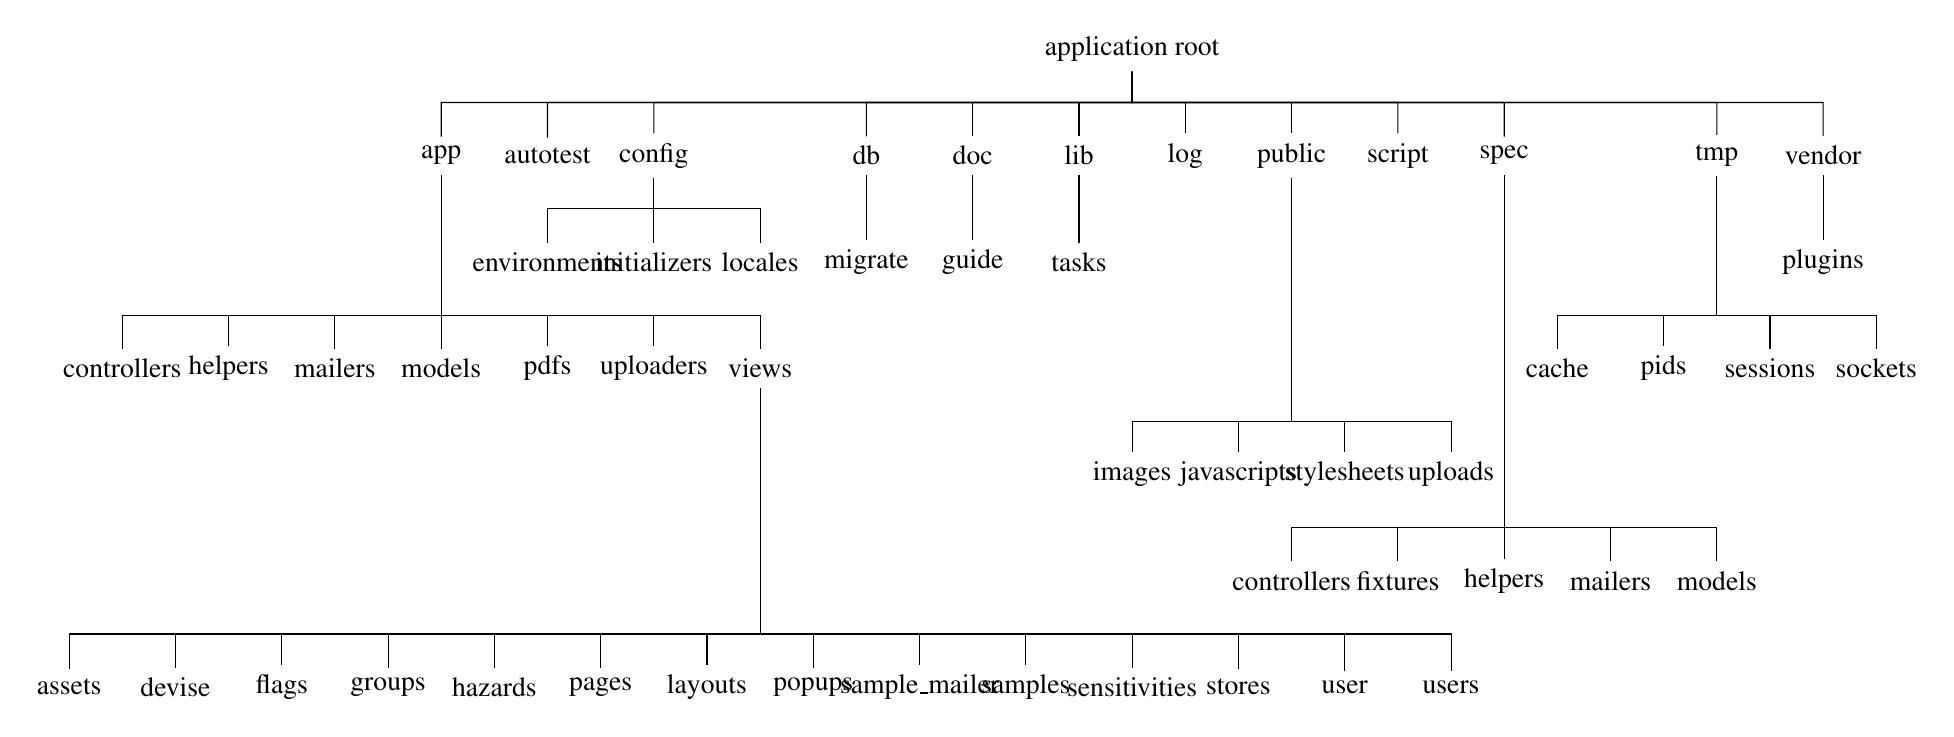
\begin{tikzpicture}[scale=0.9]
\node (root) {application root}
  [edge from parent fork down]

  child {node {app}
  child {
    child {node {controllers}}
    child {node {helpers}}
    child {node {mailers}}
    child {node {models}}
    child {node {pdfs}}
    child {node {uploaders}}
    child {node {views}
    child {
    child {
      child {node {assets}}
      child {node {devise}}
      child {node {flags}}
      child {node {groups}}
      child {node {hazards}}
      child {node {pages}}
      child {node {layouts}}
      child {node {popups}}
      child {node {sample\_mailer}}
      child {node {samples}}
      child {node {sensitivities}}
      child {node {stores}}
      child {node {user}}
      child {node {users}}
}
}
}
}
}
%  child [missing] {}
  child {node {autotest}}
  child {node {config}
    child {node {environments}}
    child {node {initializers}}
    child {node {locales}}
}
  child [missing] {}
  child {node {db}
    child {node {migrate}}
}
  child {node {doc}
    child {node{guide}}
}
  child {node {lib}
    child {node{tasks}}
}
  child {node {log}}
  child {node {public}
  child {
  child {
    child {node {images}}
    child {node {javascripts}}
    child {node {stylesheets}}
    child {node {uploads}}
}
}
}
  child {node {script}}
  child {node {spec}
  child {
  child {
  child {
    child {node {controllers}}
    child {node {fixtures}}
    child {node {helpers}}
    child {node {mailers}}
    child {node {models}}
}
}
}
}
  child [missing] {}
  child {node {tmp}
  child {
    child {node {cache}}
    child {node {pids}}
    child {node {sessions}}
    child {node {sockets}}
}
}
  child {node {vendor}
    child {node {plugins}}
}
;
\end{tikzpicture}
\normalsize
\end{center}
\vspace{1cm}
\caption{The application directory structure. Only directories are
shown here. See text for a detailed explanation.
\label{fig:filestructure}}
\end{sidewaysfigure}

The application root directory contains the following files:
\begin{verbatim}
config.ru Gemfile Gemfile.lock README.markdown
\end{verbatim}
\verb=README.markdown= is a brief summary of the application, written in
\emph{markdown}, a simple markup language similar to Textile. The
contents of this file are automatically displayed when viewing the home
page of the application on GitHub.

\verb=config.ru= is a file used to initialise the application via a
special software interface called \emph{Rack}\footnote{Rack is part
of the interface between a rails application and a web server.}.

\verb=Gemfile= contains a list of gems required to run the application.
\verb=Gemfile.lock= contains a list of all gems and their dependencies
and is used to update or install additional gems for the application.
In practice, only the \verb=Gemfile= is actually edited.

There are 12 directories directly under the application root:
\subsubsection{The app Directory}
This directory contains the bulk of the application code and templates 
for most of the page views. It contains the following subdirectories:
\begin{description}
\item[controllers]
as its name implies contains code which \emph{controls} the interface
between the database and the browser. Each table in the database has its
own controller code stored in a file in this directory. So, for example, the
controller code for access to the samples table is contained in the file
\verb=samples_controller.rb=. The \verb=.rb= extension indicates that this
file contains ruby code.
\item[helpers]
contains so-called `helper' functions (again written in ruby) which are
used to produce page views. Generally, there is a file of helper
routines corresponding to each database table, for example the helper
code containing routines to aid the display of sample data is stored in
the file \verb=samples_helper.rb=. Other files, such as
\verb=application_helper.rb= are more general-purpose and can be accessed
more widely, not just to facilitate page display for particular database
table items.
\item[mailers]
contains code used by the Rails mail subsystem. In the sample tracking
application, when samples are updated, an email is sent to relevant users.
The file \verb=sample_mailer.rb= contains the ruby code which sends the
email.
\item[models]
is one of the most important directories because it contains the code
which interacts with the database. In Rails, each database table defines
a `model' and the code to access this model is contained in a file in the
\verb=models= directory. In the case of the samples model for example, this
file is called \verb=sample.rb=.
\item[pdfs]
contains code to generate PDF versions of model data. Only sample data is
rendered to PDF form in this application. The rendering code (using the
Prawn library) is contained in the file \verb=sample_pdf.rb=.
\item[uploaders]
contains code for uploading files to the server. For each upload type, there
is a file containing the appropriate code for that file type (although
often the code will be almost identical in many cases). The standard
naming convention
for these files is \verb=<uploader_name>_uploader.rb=. For example, in the
case of an \emph{asset} upload, the code to do this is stored in the
file \verb=document_uploader.rb= because the \emph{asset} model has
a field value called \emph{document} which has been declared in its model
code as an uploader called \emph{document}\footnote{Note here that it is
the uploader name which determines the name of the file containing the
uploader code, not the field name. In this case the two are equal, but
they don't have to be.}.
Other uploader file types include zip data files, sample images and
synthetic route diagrams.
\item[views]
contains template HTML code for displaying page views of data from the
database. As can be seen from Figure \ref{fig:filestructure}, the views
directory itself contains lots of subdirectories. each subdirectory
corresponds to a model from the sample database and contains the view
templates for various different types of view associated with that model.
Let us look at the central model in the system, the \emph{sample} model.
A listing of the \verb=sample= subdirectory shows the following files:
\begin{verbatim}
dlsqueue.html.erb     groupindex.html.erb  refqueue.html.erb
edit.html.erb         index.html.erb       show.html.erb
findbarcode.html.erb  new.html.erb         userindex.html.erb
_form.html.erb        queue.html.erb
\end{verbatim}
These files all contain a mixture of traditional HTML and embedded ruby
--- hence the \verb=.html.erb= extension. Some of the files are specific
to the sample model but others are common to other models. In particular,
the files (omitting the extension) \verb=new=, \verb=show= and \verb=edit=
are templates for the \emph{create}, \emph{read} and
\emph{edit} operations.
Additionally, \verb=_form= is a form template for editing or entering 
model data. This form template is actually included by the new and edit
templates.
To get an idea of how this works, here is the edit template contained
in the file \verb=edit.html.erb=:

\scriptsize
\begin{verbatim}
<% title "Edit Sample #{@sample.code}" %>

<%= render 'form' %>

<p>
  <%= link_to "Show", @sample %> |
  <%= link_to "View All", samples_path %>
</p>
\end{verbatim}
\normalsize

Note that there are familiar HTML elements such as the paragraph tags
\verb=<p>= and \verb=</p>=. Text within the \verb=<%= and \verb=%>=
tags is ruby code. Note in particular the \verb=render 'form'= directive.
This reads in the content of the file \verb=_form.html.erb=.

Also contained in the \verb=views= directory are the email templates used
when sending confirmation/update notifications to users. These 
templates are contained in the \verb=sample_mailer= subdirectory.
There are four template files:
\begin{verbatim}
sample_receipt.html.erb  sample_update.html.erb
sample_receipt.text.erb  sample_update.text.erb
\end{verbatim}
The files contain templates for both simple text and HTML formatted emails
corresponding to emails sent on sample submission (a receipt email)
and emails sent when a sample status is updated (an update email).
Here is a listing of the template for a receipt email with HTML
formatting:

\tiny
\begin{verbatim}
<p>
Dear User
</p>

<p>
New Sample Submission Code: <%=@sample.code%> (your ref <%=@sample.userref%>)<br />
Submitted By: <%="#{@sample.user.firstname} #{@sample.user.lastname}"%>
</p>

<p>
your sample analysis request has been received. Please download a
receipt using the link below. Please quote the sample code in any
correspondence. 
</p>

<p>
There is a tear-off slip at the bottom
of the receipt which you should attach to your sample.
You will be informed via email of any
changes in the status of your sample.
</p>

<p>
<%= link_to "Analysis Request Receipt", "#{sample_url(@sample, :host => MAIL_HOST)}.pdf" %>
</p>

<p>
Copies of this email are sent to both sample submitters and their
research group leaders (where different).
</p>

<p>
Newcastle Crystallography Service
</p>
\end{verbatim}
\normalsize

Note the HTML formatting elements, \verb=<p>= and \verb=</p>= as well
as some embedded ruby (between the \verb=<%= and \verb=%>= tags).
The text version is similar, but without the HTML formatting tags.

\begin{plainblock}
You can edit the view templates without needing to restart
the application. However, large-scale changes to views should be
incorporated into the official source code repository on GitHub
(see section \ref{sec:github}).
\end{plainblock}

\end{description}
\subsubsection{The public Directory}
This directory contains files that can be \emph{directly} viewed by
a web browser. For example, if you create a file called \verb=info.html=
in this directory then (provided its permissions are suitable) you will be
able to view its contents simply by entering the following URL into your
web browser:
\begin{verbatim}
http://crystal.ncl.ac.uk/info.html
\end{verbatim}
The public directory contains things such as stylesheets, error pages
corresponding to the standard HTTP error codes\footnote{404 and 500 refer
to 'file not found' and 'internal server error' respectively. A 500 error
often arises when a program script malfunctions or there is a 
database problem.} 404, 422 and 500, generic
images (e.g. icons for buttons and logos), javascript files and any files
which are uploaded to the server. 

This last category includes all file
uploads to do with samples and assets. These files are all placed in
a directory called \verb=uploads= within the public directory.
Uploaded files are further organised depending on whether they are to
do with samples or whether they are a generic asset.
An example will best illustrate this. Suppose that a zip file of sample
analysis data is uploaded by an administrator. He is free to give the zip file
any name. Suppose he calls the file \verb=results.zip=. Then, when the file
is uploaded via the sample edit form, it will be placed in the
following location:
\begin{verbatim}
public/uploads/sample/zipdata/62/results.zip
\end{verbatim}

Similarly, a synthetic route image file called \verb=synthroute.png=
 uploaded by a user when submitting a 
sample analysis request, will be placed in the file:
\begin{verbatim}
public/uploads/sample/synth/<sample_id>/synthroute.png
\end{verbatim}
where \verb=<sample_id>= is the id automatically assigned by the database
engine to that particular sample\footnote{In fact another file will be
automatically created in the same directory, this file is a thumbnail
version of the user's file and will be given a similar name to that
which the user submitted except prefixed by the string \texttt{thumb\_}.}.
To summarise, the general form of the file path for uploaded files is:
\begin{verbatim}
<application root>/public/uploads/<model>/<uploader>/<id>/<file name>
\end{verbatim}

\subsubsection{The config Directory}\label{sec:parameters}
This directory contains configuration and initialization files
for the rails application. You will rarely, if ever need to edit most
of these. However, there is one file, \verb=environment.rb=, which
contains some parameters that you may want to change occasionally.
Here is a listing of this file (linefeeds have been added for clarity but
do not appear in any of the string variables):

\small
\begin{verbatim}
# Load the rails application
require File.expand_path('../application', __FILE__)

# Initialize the rails application
SampleTracker::Application.initialize!
ITEMS_PER_PAGE = 10 # default num items per page for will_paginate

###################  SPECIFIC GLOBAL VARS ####################
TEXTILE_REF_URL = "http://redcloth.org/textile/"
CRYS_EMAIL = "xray.cryst@ncl.ac.uk"
LOCAL_ADMIN_EMAIL = "crysadmin@milkyway.ncl.ac.uk"
TEXTILE_QUICK_REF_URL = "http://en.wikipedia.org/wiki/Textile_%28markup_language%29"
SAMPLE_INTRO_TEXT = "a unique code and a barcode will be
automatically generated on submission of this form when a new sample
is created. For synthetic route files, please use either the JPG or PNG
bitmap image format.
Note further that for security reasons, if there are validation errors
in the form, you will have to re-select the names of uploaded files.
Also remeber to set the priority number, the form will not validate unless
you do this (if you are not going to submit several samples in a short
space of time we suggest setting the priority number to 1)."
QUEUE_INTRO_TEXT = "The following gives an appoximate wait time before your 
sample will be analysed. The actual time will vary depending on sample 
quality and priority number."
DLS_VISIT_DATE = "31/06/2012"
DLS_QUEUE_INTRO_TEXT = "The following samples are awaiting analysis at the 
Diamond Light Source (DLS). The next visit to DLS is 
scheduled for #{DLS_VISIT_DATE}."
REF_QUEUE_INTRO_TEXT = "The following samples are awaiting further refinement after initial data collection."
\end{verbatim}
\normalsize

There are several constants (those parameters in capitals) which define
parameters which affect the way the application runs:
\begin{description}
\item[\texttt{\textbf{ITEMS\_PER\_PAGE}}]
is the parameter that controls the \emph{default} pagination of lists
as mentioned elsewhere. Lists will use this parameter as a default, but
in most cases users can change the pagination on-the-fly.
\item[\texttt{\textbf{TEXTILE\_REF\_URL}}]
contains a URL pointing to a complete Textile reference --- currently
it refers to the RedCloth web site.
\item[\texttt{\textbf{CRYS\_EMAIL}}]
is the email account to which sample submission requests are sent.
\item[\texttt{\textbf{LOCAL\_ADMIN\_EMAIL}}]
this is set to the email address which appears in the \emph{From}
part of all emails which are automatically sent to users by the sample
tracking system.
\item[\texttt{\textbf{TEXTILE\_QUICK\_REF\_URL}}]
contains a URL to a Textile quick reference page. This is currently set
to the Wikipedia entry for Textile and is used on the page edit screen
to help administrators edit static pages as shown in Figure \ref{fig:editpage}.
\item[\texttt{\textbf{SAMPLE\_INTRO\_TEXT}}]
contains the text that appears at the beginning of the sample
submission form --- see for example Figure \ref{fig:sampleeditform}. 
\item[\texttt{\textbf{QUEUE\_INTRO\_TEXT}}]
contains the text that appears in a box at the beginning of the sample
queue page.
\item[\texttt{\textbf{DLS\_VISIT\_DATE}}]
contains the date of the next visit to the \emph{Diamond Light Source}. This
parameter will often be referenced in other global variables and view files.
For example, the \verb=DLS_QUEUE_INTRO_TEXT= variable in the listing above
refers to this variable.
\item[\texttt{\textbf{DLS\_QUEUE\_INTRO\_TEXT}}]
contains the text that appears at the beginning of the DLS sample
queue page.
\item[\texttt{\textbf{REF\_QUEUE\_INTRO\_TEXT}}]
contains the text that appears at the beginning of the refinement sample
queue page.
\end{description}

\begin{plainblock}
Note that if any of these parameters are changed, the server will need
to be restarted before the changes will take effect. You should also
make a note of such changes in the case of a system upgrade because
the source code on GitHub will not necessarily have these parameters
set to the same values.
\end{plainblock}

\subsubsection{The db Directory}
This directory contains the actual database used in the application.
The production database is stored in a single file, \verb=production.sqlite3=.
There may also be a development database, \verb=development.sqlite3= used
for development work. The latter file is never used in a production environment
however. One other important file is \verb=schema.rb=. This is a file
containing ruby code which can be used to re-generate the entire blank
database schema.

There is also a directory called \verb=migrate=. This contains all of the
\emph{migrations} which have been applied to the database since it was
first initialised. A migration is simply an adjustment to the database
schema. For example, you may create an initial table in the database but
later realise that you want to change some characteristic of the table
such as adding an extra field or changing the datatype of an existing field.
You can do this by setting up a migration --- basically a bit of ruby code
which will perform the necessary changes. 
The file \verb=schema.rb= mentioned earlier can be
thought of as an accumulation of all the migrations that have been applied
to the database to get it to its current state.

\subsubsection{Other Directories}
There are several other directories:
\begin{description}
\item[tmp]
holds temporary files created by \samtrack.
This directory has subdirectories for storing
cache contents, session information and sockets. These files are automatically
cleaned up from time-to-time although an occasional manual clean-out may be
necessary if things go wrong.
\item[doc]
contains documentation of various sorts.
The subdirectory \verb=guide= contains this administrator's guide as well
as the \LaTeX\ source file and included figures needed to create it.
There are also several markdown formatted files which contain 
informally-written information about the development of the application.
\item[spec]
is not used at present. It is intended as the location for
a complete testing suite for the application. The test suite has not yet
been written, but may be in the future.
\item[autotest]
is intended to hold files related to automatic testing.
It is not used at present.
\item[lib]
contains code that doesn't neatly fit anywhere else.
Within this directory is a file called 
\verb=development_mail_interceptor.rb=
which is used to set up an email environment in development mode, where
you don't want emails to be sent to actual users. The code in this file
redirects all email to a specific developer's email address.
There is also a \verb=tasks= directory used to put code for any
Rake\footnote{Rake is a \emph{build tool} which is used by developers to
automate certain tasks. It is also used within rails to perform database 
migrations.} tasks which have been written by developers. No custom
Rake tasks have been written for this application so the directory is
currently empty.
\item[log]
contains special development log information.
\item[vendor]
is the place where third-party code can be stored. It has a subdirectory,
\verb=plugins= where extensions to rails are stored. Plugins
extend core rails functionality. We don't use any rails plugins in this
application at the moment so the directory is empty. The \verb=vendor=
directory can also be used to store rails and all of its dependencies
rather than relying on the operating system to provide them. At present
we don't use this feature, but in future, when the application is stable,
this is probably where we will install an independent copy of rails and
its dependent software (e.g. gems) in order that the whole application
is autonomous and not reliant on what the operating system provides.
\end{description}

\subsection{Web Server Management}
Most of the time, you should need only
two commands when managing the web server --- the commands to switch it on
and off. To do this use:
\begin{verbatim}
sudo apache2ctl start|stop
\end{verbatim}
You would typically stop the server to do some maintenance such as editing
a stylesheet or a major upgrade to the software.
Occasionally you may need to change some server parameters in the
web server configuration files. The main configuration file is
\verb=/etc/apache2/apache2.conf=. You will rarely, if ever, need to
change anything here unless you want to tweak the server performance (in
which case you'll definitely need to know what you're doing). This file
does contain some parameters for the apache \emph{Phusion Passenger} 
module which is needed to interface Rails with the apache server:
\begin{verbatim}
LoadModule passenger_module /usr/local/rvm/gems/ruby-1.9.2-p290/
gems/passenger-3.0.9/ext/apache2/mod_passenger.so
   PassengerRoot /usr/local/rvm/gems/ruby-1.9.2-p290/gems/passenger-3.0.9
   PassengerRuby /usr/local/rvm/wrappers/ruby-1.9.2-p290/ruby
\end{verbatim}
These configuration lines are added as part of the installation of
\emph{Phusion Passenger} and tell it where the ruby interpreter and
passenger software reside in the file system.

The \verb=apache2.conf= file also contains a line which refers to some other
configuration files:
\begin{verbatim}
Include /etc/apache2/sites-enabled/
\end{verbatim}
The above line tells the server to get some further configuration
details from the contents of the directory
\verb=/etc/apache2/sites-enabled=.
\verb=sites-enabled= contains a file called \verb=000-default= which contains
the descriptions of all the \emph{virtual hosts}\footnote{A single Apache
web server can support multiple so-called virtual hosts which behave as
separate web sites.}. The most important virtual host entry is the one
for the host \verb=crystal.ncl.ac.uk=. Here is the entry in full:
\begin{verbatim}
<VirtualHost *:80>
      ServerName crystal.ncl.ac.uk
      DocumentRoot /usr/local/share/sample_tracker/public
      <Directory "/usr/local/share/sample_tracker/public">
         AllowOverride all
         Options -MultiViews
      </Directory>
        ErrorLog /var/log/apache2/error-crystal.log
</VirtualHost>
\end{verbatim}
For virtual hosting to work, any name given to a virtual host
(e.g. in this case \verb=crystal.ncl.ac.uk=) must be an official alias
for the actual apache web server (in this case \verb=milkyway.ncl.ac.uk=).
We will now describe in detail what these directives mean.

The first line is a tag which defines the beginning of a virtual host
definition. It has the form \verb=<VirtualHost *:80>=. The number \verb=80=
is the \emph{port number}\footnote{A port number defines a communications
channel between computers on the Internet. Port 80 is usually
used by the HTTP protocol for communication between web servers and browsers
although other port numbers can be used.}.
The last line is a closing tag, \verb=</VirtualHost>=. the lines in-between
contain the directives which control the configuration of this host.
\begin{description}
\item[\texttt ServerName]
This directive sets the name of the virtual host, in this case
\verb=crystal.ncl.ac.uk=.
\item[\texttt DocumentRoot]
Sets the absolute path of the directory on the server which contains
all static documents which can be \emph{directly} viewable on a web browser.
No documents outside this directory can be viewed directly or downloaded.
In this case, the document root is 
\verb=/usr/local/share/sample_tracker/public=
i.e. the \verb=public= directory within the root \samtrack\ directory.
This is a standard rails convention.
\item[\texttt ErrorLog]
Specifies the absolute path of the error log file for this virtual host.
Here, it is set as \verb=/var/log/apache2/error-crystal.log=.
\end{description}
There is also a \verb=Directory= section in the virtual host definition.
This has the form of an opening and closing tag with directives in-between.
The opening tag has an argument which is the full path of the particular
directory to which the directives apply. Note that the argument is in quotes.
In this case the argument is the same directory as the document root.
Note further that there may be more than one \verb=Directory= section.
The directives are as follows:
\begin{description}
\item[\texttt AllowOverride]
This directive controls whether directives contained in a file
(conventionally called \verb=.htaccess= contained in a particular
directory can override earlier configuration directives at the server
configuration level. The argument refers to which type of directive
can be overridden --- in this case \verb=all=.
\item[\texttt Options]
This sets a number of options when viewing files contained in the
relevant directory. here, we have set the \verb=-MultiViews= option
which allows a single document to be displayed in different ways dependent
on browser capabilities.
\end{description}

\begin{plainblock}
\begin{center}
\bfseries Root Directory Location of \samtrack
\end{center}
It should be clear from the above that if you want to change the root
directory of \samtrack\  you must edit the
virtual host directive file and change the \verb=DocumentRoot= directive
and \verb=Directory= section argument appropriately.
\end{plainblock}

We end this section on web management with a brief discussion about
file permissions. Once you have uploaded the application and all its
files to a suitable location you must make sure that the file permissions
are correct. The correct permissions for all files are to set group
ownership to \verb=root= and user ownership to \verb=nobody=\footnote{%
\texttt{nobody} is a special user account available on most linux
systems.}. This can be done with a simple one-line command:
\begin{verbatim}
sudo chown -R nobody.root <application document root>
\end{verbatim}

\subsection{Raw Database Management}
Hopefully, you won't often need to refer to this section because
\samtrack\  will handle all of the database operations
for you. Sometimes however, the database becomes broken in some way
and needs to be edited in its `raw' form. For example, you may
be logged in as an administrator and inadvertently remove your own
administration rights. If you were the only administrator then you now
have a problem because only an administrator can change a user's rights!
We will look at how to solve this particular problem later in this
section. We consider specifically SQLite3 database manipulation here
since that is the database used in the application.
In this section we describe two utilities for manipulating
SQLite3 databases, the command-line linux program \emph{sqlite3} and
the web browser plugin \emph{sqlite-manager}\cite{sqlitemanager}.

\subsubsection{Database Management with sqlite3}
\emph{sqlite3} is available on all systems where the SQLite3 database
is installed. Here, we briefly describe how to use it to manipulate the
sample database and give one example of its use in a practical situation.
A simple command gets you started:
\begin{verbatim}
sqlite3 <sqlite3 database file>
\end{verbatim}
which produces some informational output followed by a prompt:
\begin{verbatim}
SQLite version 3.6.22
Enter ".help" for instructions
Enter SQL statements terminated with a ";"
sqlite> 
\end{verbatim}
All commands in sqlite3 begin with a full stop. Assuming, we're looking
at the sample tracking database, typing \verb=.tables= will give a list
of tables in the database:
\begin{verbatim}
sqlite> .tables
assets                 pages                  schema_migrations    
flags                  popups                 sensitivities        
groups                 samples                stores               
hazards                samples_sensitivities  uploads              
hazards_samples        samples_stores         users                
sqlite> 
\end{verbatim}
The \verb=.schema= command can be used to check the schema of either
individual tables or, without an argument, \emph{all} tables:

\small
\begin{verbatim}
sqlite> .schema samples
CREATE TABLE "samples" ("id" INTEGER PRIMARY KEY AUTOINCREMENT NOT NULL, "code"
varchar(255), "cif" varchar(255), "synth" varchar(255), "coshh_name" varchar(255
), "coshh_desc" varchar(255), "coshh_info" text, "params" varchar(255), "priorit
y" integer, "powd" boolean, "chiral" boolean, "cost_code" varchar(255), "barcode
" varchar(255), "created_at" datetime, "updated_at" datetime, "user_id" integer,
 "flag_id" integer DEFAULT 1 NOT NULL, "userref" varchar(255), "zipdata" varchar
(255), "sampleimage" varchar(255), "reference" varchar(255), "comments" text, "c
olour" text, "size" text, "shape" text, "feedback" text);
sqlite> 
\end{verbatim}
\normalsize

What is displayed here is the SQL command sequence needed to create the
table (in this case the samples table). You can deduce from this the whole
table schema --- field names, data types, whether a particular field is
allowed to be NULL or if it has a default value etc.

If you want to actually enter data into or edit a database, you need to 
understand the database query language SQL. A good, quick introduction is
available on the \emph{w3schools} web site\cite{w3schoolssql}.
Now, as an example, let's return to the problem of giving a user
administration rights when there are no other such users\footnote{If you think about it, this will always be the case initially!}.
In this case we'll use sqlite3 to give a particular user administration
rights. We'll assume that the user's last name is 'Hagon'. First, we need
to find the user. Here's the SQL to do that\footnote{Note that SQL
commands must be terminated by a semi-colon.}:

\small
\begin{verbatim}
sqlite> select * from users where lastname = 'Hagon';
2|jerry.hagon@ncl.ac.uk|$2a$10$V2eSY1MD2dWkIESZ/3mtGe8hYvVDVkDTDEd4NKqZOQJ3t9wg9
8iFq|hkTD7hHWzEu5ErjSFh2y|2012-02-16 10:19:43.792239||190|2012-04-06 07:43:02.65
2582|2012-04-04 13:58:26.642714|127.0.0.1|127.0.0.1|2011-11-06 15:18:43.971379|2
012-04-06 07:43:02.653005|19|f|Jerry|Hagon|t|t
sqlite> 
\end{verbatim}
\normalsize

Now, what does all this mean? First, each field in the output is separated
by a vertical bar (\verb=|=). The order of the fields is determined by the
schema, so let's find this out:

\small
\begin{verbatim}
sqlite> .schema users
CREATE TABLE "users" ("id" INTEGER PRIMARY KEY AUTOINCREMENT NOT NULL, "email" v
archar(255) DEFAULT '' NOT NULL, "encrypted_password" varchar(128) DEFAULT '' NO
T NULL, "reset_password_token" varchar(255), "reset_password_sent_at" datetime, 
"remember_created_at" datetime, "sign_in_count" integer DEFAULT 0, "current_sign
_in_at" datetime, "last_sign_in_at" datetime, "current_sign_in_ip" varchar(255),
 "last_sign_in_ip" varchar(255), "created_at" datetime, "updated_at" datetime, "
group_id" integer, "admin" boolean DEFAULT 'f', "firstname" varchar(255), "lastn
ame" varchar(255), "leader" boolean DEFAULT 'f', "enabled" boolean DEFAULT 't');
CREATE UNIQUE INDEX "index_users_on_email" ON "users" ("email");
CREATE UNIQUE INDEX "index_users_on_reset_password_token" ON "users" ("reset_pas
sword_token");
sqlite> 
\end{verbatim}
\normalsize

Ignoring the \verb=CREATE UNIQUE INDEX= which don't relate to the order of the
fields, we see that in the \verb=CREATE TABLE= entry (which ends with the
semi-colon before the firts line beginning with \verb=CREATE UNIQUE INDEX=)
the last five fields are \verb=admin=, \verb=firstname=, \verb=lastname=
\verb=leader= and \verb=enabled=. \verb=admin= is the key field --- it's
a \emph{boolean} field having only two values, true or false (labelled
as either \verb='t'= or \verb='f'= in the above output.

The last five entries for the user were listed as \verb=f|Jerry|Hagon|t|t=
which means that he is not an administrative user. To give this user
administrative rights we must change the \verb=admin= field (5th from last).
Here is the SQL to do that:

\small
\begin{verbatim}
sqlite> update users set admin='t' where id=2;
sqlite> select * from users where lastname = 'Hagon';
2|jerry.hagon@ncl.ac.uk|$2a$10$V2eSY1MD2dWkIESZ/3mtGe8hYvVDVkDTDEd4NKqZOQJ3t9wg9
8iFq|hkTD7hHWzEu5ErjSFh2y|2012-02-16 10:19:43.792239||190|2012-04-06 07:43:02.65
2582|2012-04-04 13:58:26.642714|127.0.0.1|127.0.0.1|2011-11-06 15:18:43.971379|2
012-04-06 07:43:02.653005|19|t|Jerry|Hagon|t|t
sqlite> 
\end{verbatim}
\normalsize
 
And we can see from the \verb=select= command that the change has been applied.
Note that we have used the SQL \emph{update} command and applied it to the
user whose \verb=id= field is 2. Now, the \verb=id= field
is the first one in the list and we have used that to refer to the user.
We could also have used any other field, but the \verb=id=  field is unique
and so is guaranteed to refer to only one user. A command such as:
\begin{verbatim}
update users set admin='t' where lastname='Hagon';
\end{verbatim}
would also work but if there were, say, two users with that same last name, 
the change would be applied to both of them.

\subsubsection{Database Management with sqlite-manager}
\emph{sqlite-manager} provides a graphical user interface to SQLite3
database management. It is a web browser plugin available for the Firefox
web browser and can be easily installed via a
simple one-click link\cite{sqlitemanager}.
The plugin is accessed via the Firefox \emph{Tools} menu as shown in
Figure \ref{fig:firefoxtools}.

\begin{figure}[!htb]
\begin{center}
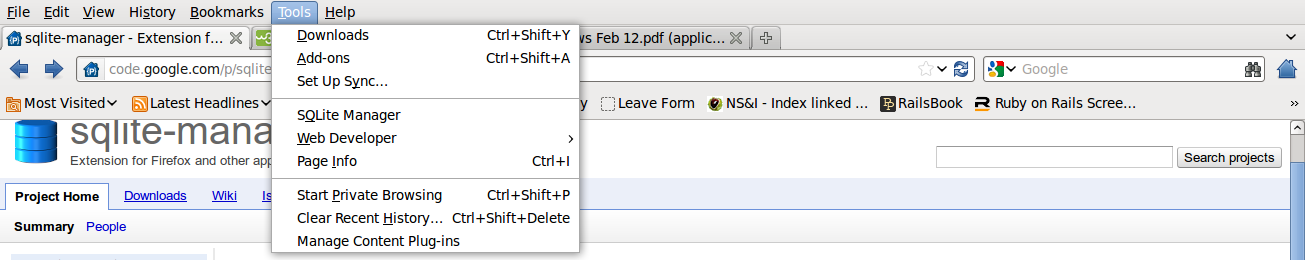
\includegraphics[width=0.95\textwidth]{firefoxtools}
\caption{Firefox \emph{Tools} menu showing the link to the installed
\emph{sqlite-manager} plugin (4th from top in the menu).
\label{fig:firefoxtools}}
\end{center}
\end{figure}

\begin{figure}[!htb]
\begin{center}
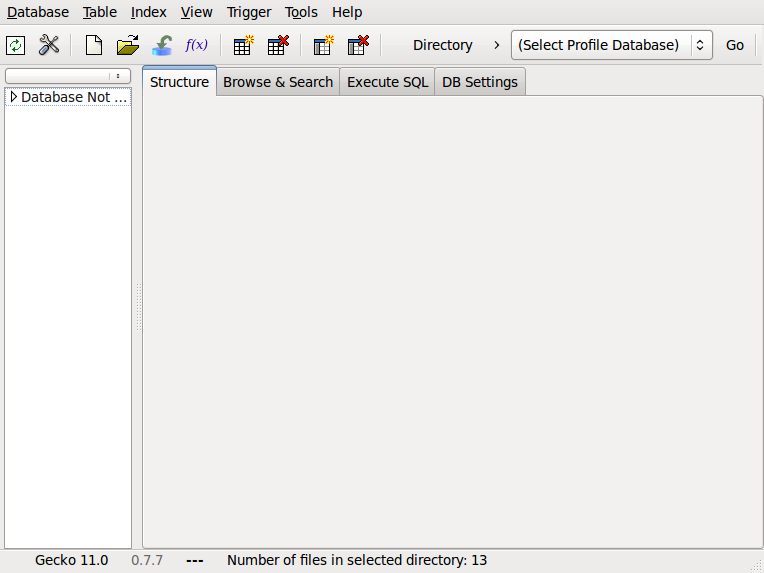
\includegraphics[width=0.75\textwidth]{sqlitemanwin}
\caption{Initially the user is presented with the main
sqlite-manager window. \label{fig:sqlitemanagerwindow}}
\end{center}
\end{figure}

When sqlite-manager starts up, you first see the main window shown
in Figure \ref{fig:sqlitemanagerwindow}.
To read in a database, select \emph{Connect Database} from the
\emph{Database} menu.
A file browser window will appear, but by default it shows only those
files with extension \verb=.sqlite=. At the bottom right of this window
is a drop-down select box which allows you to view `All Files'. After
selecting this option you will be able to see any file in the window.
After browsing to the appropriate directory and selecting the database file
you want (we will use a sample tracking database file in the description
to follow), the main window should show the database as shown in
Figure \ref{fig:sqlitemanagerdat}.

\begin{figure}[!htb]
\begin{center}
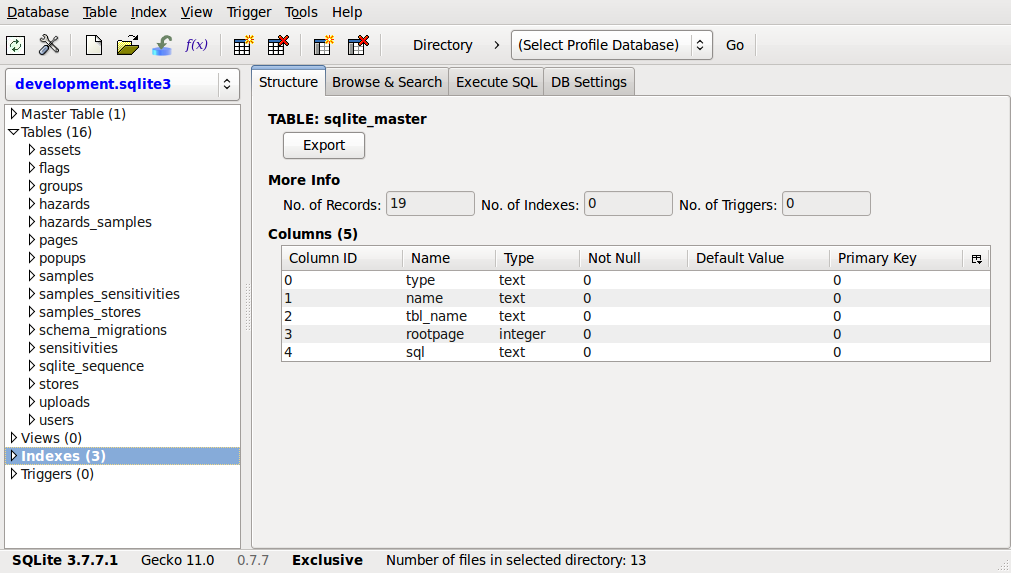
\includegraphics[width=0.75\textwidth]{sqlitemandat}
\caption{The main sqlite-manager window after loading a sample
tracking database file. Note the list of tables in the left hand panel.%
\label{fig:sqlitemanagerdat}}
\end{center}
\end{figure}

We will now try to do the same update that was performed using the
command-line utility \emph{sqlite3} previously. To begin, select the
\emph{users} table from the list in the left hand panel then select
the \emph{Browse \& Search} tab in the main panel. You should see a list
of users (you can use the mouse to adjust the width of the field columns).
This is shown in Figure \ref{fig:sqlitemanagerlist}.

\begin{figure}[!htb]
\begin{center}
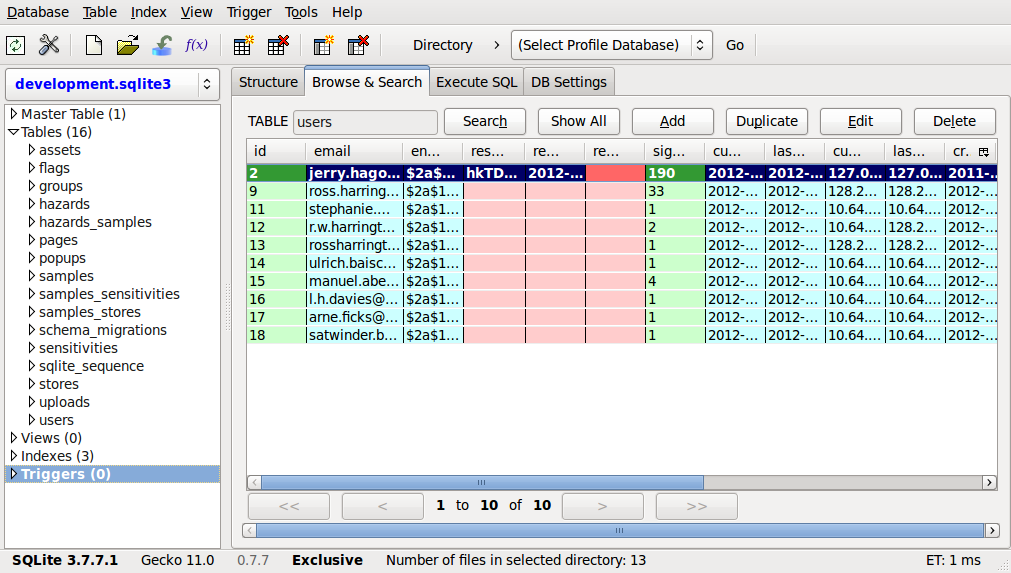
\includegraphics[width=0.75\textwidth]{sqlitemanlist}
\caption{The \emph{users} table listing in the \emph{Browse \& Search}
tab in the main panel.%
\label{fig:sqlitemanagerlist}}
\end{center}
\end{figure}

Editing an entry is easy, just double-click on the row that you want to edit
--- in this case the first one. The \emph{Edit Record} box will pop up.
Scroll down until you reach the admin field, change its value
accordingly and then click the \emph{OK} button 
(Figure \ref{fig:sqlitemanageredit}.

\begin{figure}[!htb]
\begin{center}
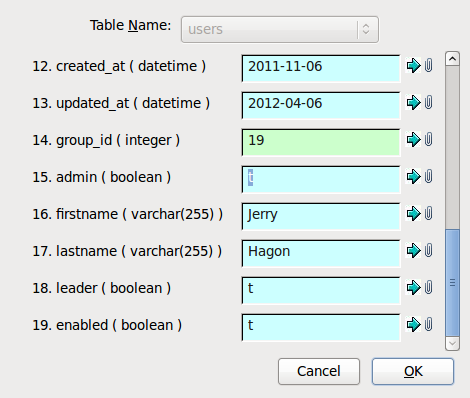
\includegraphics[width=0.45\textwidth]{sqlitemanedit}
\caption{The sqlite-manager \emph{Edit Record} window. Each field in the
record can be edited.\label{fig:sqlitemanageredit}}
\end{center}
\end{figure}

The sqlite-manager plugin is very powerful and well-worth experimenting
with (using a test database of course!). It can perform arbitrary SQL
commands via an SQL command panel and has simple short-cuts for doing
most update/create operations. There are also easy-to-use search and sort
facilities.

There are other tools which can be used to manipulate SQLite3 databases.
The two we have described are freely available. Other free alternatives
are also available as well as commercial tools. Some of these are described
on the SQLite web site.

\subsection{Software Updates and GitHub}\label{sec:github}
The \samtrack\ application is stored on GitHub\cite{github}, a
a web-based hosting service for projects that use the 
\emph{Git} revision control system.
This means that the source code is safe and new versions of the
software can be quickly downloaded and installed.
Anyone can view the \samtrack\ repository. 
The URL is \url{https://github.com/jhagon/sample_tracker}.
Typing this URL into your browser produces a page something like that
shown in Figure \ref{fig:github1}.

\begin{figure}[!htb]
\begin{center}
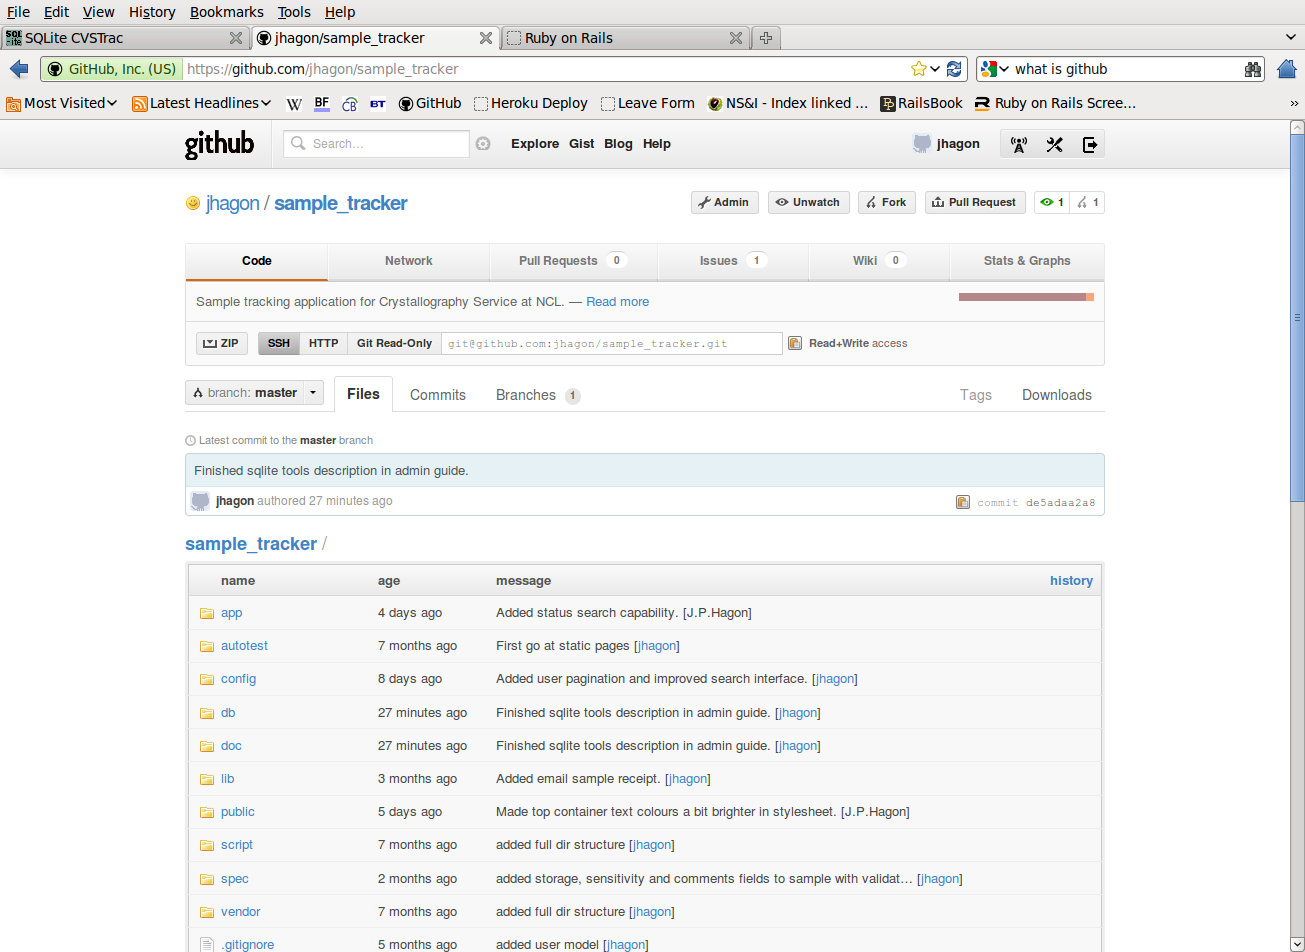
\includegraphics[width=0.75\textwidth]{github1}
\caption{The \samtrack\ GitHub repository.\label{fig:github1}}
\end{center}
\end{figure}

The GitHub repository contains a wealth of information about the
development of the software and its current status. You can browse
the entire file structure of the system, downloading individual files
or the entire repository. Any development work on the system will be
mirrored on GitHub so that the latest version of the software can be
downloaded at any time. It is also possible to download any previous
version of the software if needed.

To download the current version of \samtrack, simply click on the
\emph{ZIP icon} near the top of the file browser panel on the left hand side. 
This will
pack the whole of the source into a compressed ZIP file. If you
require a specific version, then first click the \emph{history} link on the
top right of the main file browser panel. This will take you to the
\emph{Commit History} page. If you click on the descriptive text for
a particular revision, you will be taken to the summary page for that
particular revision. Near the top right is a \emph{Browse code} button
which when clicked will take you to a file browser panel for that revision.
Again, you will see a \emph{ZIP icon}, on the top-left of the file browser
panel which you can click to get a ZIP file of that version.

You can also submit bug reports via the GitHub page although you must
be registered to do so. Current issues can be viewed via the link at
the top of the main repository page.
Also, there are statistics and charts which provide detailed information
about the application.

\subsection{Backup and Upgrade Procedures}
It is essential of course to make sure that the system is adequately
backed-up. As we have seen, a copy of the software itself (both current
and previous versions) is safely stored on GitHub. However, GitHub
does not store sample data --- you must take steps to make sure the
sample data is safe. As a general rule, if you back up the whole of the
application root directory then that is sufficient. 
As mentioned in section \ref{sec:parameters} you should also make
a note of any global parameters that you change because these will
not necessarily be reflected in the GitHub source if you perform
a full upgrade of \samtrack. 

Volatile sample data is stored in two places:
\begin{enumerate}[(i)]
\item
The SQLite3 database file
\verb=<application root>/db/production.sqlite3=;
\item
The public directory
\verb=<application root>/public= and everything underneath it.
\end{enumerate}

\subsubsection{System Upgrade Procedure}\label{sec:upgrade}
There are two circumstances where you will need to do a full system upgrade:
\begin{itemize}
\item
after major updates to the software;
\item
whenever the database schema has changed (no matter how small the change
may be).
\end{itemize}

\begin{plainblock}
\begin{center}
\bfseries Database Schema Changes
\end{center}
Schema changes can be very minor, e.g. a renaming of a field, a change
in data type, a change in default value etc. or they can be more complex, 
such as the
addition of one or more fields or even whole new tables. However, a schema
change \emph{no matter how small} necessitates a full system upgrade in
the manner described below.
\end{plainblock}


We will go through the steps needed to perform a full
software upgrade. This procedure is also described in the file
\verb=<application root>/doc/UPGRADE.markdown=\footnote{If you view
this file (and any other markdown-formatted file) on GitHub, it will
be nicely formatted according to the markdown specifications.}

\begin{enumerate}
\item
login using the \verb=crysadmin= account and switch to a root shell:
\begin{verbatim}
sudo bash
\end{verbatim}
\item
Stop the web server:
\begin{verbatim}
apache2ctl stop
\end{verbatim}
\item
Change to the directory which contains the \samtrack\ application 
(usually \verb=/usr/local/share=) and
move the application root directory to a different place thus retaining a
complete copy of the old system --- we don't want to scrub it just in case!
\begin{verbatim}
cd /usr/local/share
mv sample_tracker sample_tracker.old
\end{verbatim}
\item
Go to the GitHub repository where the latest copy of the application is stored
and download a copy using the procedure described in section
\ref{sec:github}. Put the downloaded ZIP file in a temporary directory
such as \verb=/tmp=. The ZIP file will have a name similar to
\verb=jhagon-sample_tracker-b493e1b.zip= with the \verb=b493e1b= part
indicating the revision:
\begin{verbatim}
mv jhagon-sample_tracker-b493e1b.zip /tmp
\end{verbatim}
\item
Now, unzip the file in the temporary directory 
(at the moment, it doesn't matter where you do this):
\begin{verbatim}
unzip jhagon-sample_tracker-b493e1b.zip
\end{verbatim}
You should have a directory called something like:
\begin{verbatim}
jhagon-sample_tracker-b493e1b
\end{verbatim}
tem
Move the above directory to the live application location:
\begin{verbatim}
mv jhagon-sample_tracker-b493e1b /usr/local/share
\end{verbatim}
then change to the \verb=/usr/local/share= directory and rename the\newline
\verb=jhagon-sample_tracker-b493e1b= directory to \verb=sample_tracker=:
\begin{verbatim}
cd /usr/local/share
mv jhagon-sample_tracker-b493e1b sample_tracker
\end{verbatim}
\item
Change to the \verb=sample_tracker= directory and remove the production 
database (if it exists) and also the \verb=public= directory:
\begin{verbatim}
rm db/production.sqlite3
rm -rf public
\end{verbatim}
\item
Now we must import the live production database and \verb=public=
directory from the saved copy of the previous application:
\begin{verbatim}
cp <previous sample_tracker dir>/db/production.sqlite3 db
cp -r <previous sample_tracker dir>/public .
\end{verbatim}
where the above commands are assuming we're in the new application root
directory (\verb=/usr/local/share/sample_tracker=).
If the database schema has not changed, go to step 
\ref{item:num}. Otherwise:
\item
We must now migrate the database to its new schema. First we must make
sure we are running the latest ruby. The server's default version of ruby is
too old so we must instead use a special version which we can access by
typing:
\begin{verbatim}
source /etc/profile.d/rvm.sh
\end{verbatim}
to check this, if you type `ruby -v` you should get something
similar to this --- the important part is the version number of ruby,
it should be 1.9.x:
\begin{verbatim}
ruby 1.9.2p290 (2011-07-09 revision 32553) [i686-linux]
\end{verbatim}
\item
Now perform a database schema migration by typing the following:
\begin{verbatim}
export RAILS_ENV=production
rake db:migrate
\end{verbatim}
Note that you may see a couple of warnings during the rake command, but
this is OK.
\item\label{item:num}
We are almost done. Next change the ownership of the entire 
\verb=sample_tracker=
directory structure to user \verb=nobody=. Before doing this we change
directory to that which holds the application root directory:
\begin{verbatim}
cd /usr/local/share
chown -R nobody.root sample_tracker
\end{verbatim}
\item
Now all that is left is to start the web server (and hope!):
\begin{verbatim}
apache2ctl start
\end{verbatim}

\end{enumerate}

At this point you should perform a few checks on the new system. If there are
problems, you can stop the web server, scrub the new version and copy the 
previous saved version back to the correct location. then restart the web
server.


\section{Database Schema Description}\label{sec:database}
\subsection{Introduction}
The core of the system is the database which holds information about 
users, samples etc. In this section we describe the whole database
structure (or \emph{schema} in database parlance) at the time
of writing.
The easiest way to get an overall view of the database schema is to
study Figure \ref{fig:database_schema}. This shows
all the tables, fields and relationships in a single diagram.
We now give a brief description of each table.

Note that all tables except join tables have an auto-incremented integer field
called \verb=id= which servers as the unique primary key for each record
in the table. The \verb=id= field will not be listed explicitly in the
description of each table. All non-join tables also have two other
fields, \verb=created_at= and \verb=updated_at= in a datetime format.
Again, we will not explicitly list these fields in the description
of the tables which follows.

\subsection{The Samples Table}
The samples and users tables are the key parts of the database as is
evident from Figure \ref{fig:database_schema}. They are related to each
other via a \emph{one-to-many} relationship, i.e. \emph{one} user
can have \emph{many} samples but a single sample is associated with
just \emph{one} user. The samples table consists of the following fields:
\begin{description}
\item[code]
a string, automatically generated by the system having the
general form \verb=AAA-AA-YY-1111= where the \verb=AAA= and \verb=AA= 
represent 3-letter codes for group and submitter respectively; 
the \verb=YY= represents the year and the \verb=1111= represents a number 
which is incremented for that group but reset to zero at the start of each 
calendar year.
\item[cif]
a string representing the chemical formula of the sample in cif format.
\item[synth]
a string representing the file name of an image file specifying the details
of the synthesis.
\item[coshh\_name]
a string representing the name of the solvent (if any).
\item[coshh\_info]
another string describing any procedures in case of contact with the sample.
\item[coshh\_desc]
a text field providing a brief description of the sample (e.g. organic amide).
\item[params]
a string representing unit cell parameters
or CSD/Newcastle code for possible by-products or previously obtained, 
unpublished results.
\item[priority]
an integer between 1 and 9 to give an indication of priority.
\item[powd]
a boolean parameter indicating if the sample requires powder diffraction (y/n).
\item[chiral]
another boolean indicating whether the molecule is chiral (y/n).
\item[costcode]
a string providing a cost centre code for charging if relevant.
\item[barcode]
a string field for an automatically generated Code39 standard bar code.
\item[user\_id]
this integer holds the \verb=id= field of the user who requested the
sample analysis.
\item[flag\_id]
an integer holding the \verb=id= field of the status flag of the sample.
\item[userref]
a string for a user-defined reference. This is required to be an
alphanumeric sequence of characters \emph{without spaces}.
\item[zipdata]
a string holding the name of a zip file containing the results of the analysis.
\item[sampleimage]
a string holding the name of an image file of the sample molecule after it
has been identified by the analysis.
\item[reference]
a text field for a published reference (typically in the form of a DOI).
\item[comments]
a text field for any general comments the user wishes to make about the sample.
\item[colour]
a string holding information about the colour of a sample after analysis.
\item[size]
a string holding information about the size of a sample after analysis.
\item[shape]
a string holding information about the shape of a sample after analysis.
\item[feedback]
a text field containing any additional comments on the sample by
crystallography staff.
\end{description}

\subsection{The Users Table}
The users table, in addition to maintaining a record of users and their
samples, also serves as a key part of the authentication and authorisation
system which will be described later. the users table is related to the
samples table via a \emph{one-to-many} relationship, i.e. \emph{one} user
has \emph{many} samples.
\begin{description}
\item[email]
a string holding the email address of the user. This serves also as the
user login id.
\item[encrypted\_password]
a string holding the user's password in an encrypted form.
\item[reset\_password\_token]
a string containing a special token used if the user has forgotten his
password and needs to reset it.
\item[reset\_password\_sent\_at]
a datetime field recording the time a token enabling a user to reset his
password was sent.
\item[remember\_created\_at]
a datetime field specifying the time at which a user requested that his
login id be remembered by the browser so he need not type in his credentials.
\item[sign\_in\_count]
an integer holding the number of times a user has logged-in.
\item[current\_sign\_in\_at]
a datetime field holding the sign-in time for the current session.
\item[last\_sign\_in\_at]
a datetime field holding the last sign-in time for the user.
\item[current\_sign\_in\_ip]
a datetime field holding the user's ip address for the current session.
\item[last\_sign\_in\_ip]
a datetime field holding the previous login ip address for the user.
\item[group\_id]
an integer representing the \verb=id= field of the group to which
the user belongs.
\item[admin]
a boolean field indicating whether the user is an administrator (y/n).
\item[firstname]
a string holding the user's first name.
\item[lastname]
a string holding the user's last name.
\item[leader]
a boolean field indicating whether the user is a group leader (y/n).
\item[enabled]
a boolean field indicating if the account is enabled (y/n).

\end{description}

\subsection{The Stores, Hazards and Sensitivities Tables}
These tables are each very similar and have the same basic structure.
They are used to specify storage, hazard and sensitivity properties
for a sample. They all have a \emph{many-to-many} relationship with
the samples table. This is because a sample can have, for example,
\emph{many} storage requirements, but also a single storage requirement
can be associated with \emph{many} samples.
All these tables have essentially the same fields:
\begin{description}
\item[name]
a string defining a short name for the property.
\item[description]
a text field describing the property at greater length.
\end{description}
For historical reasons, the hazards table uses the names
\verb=hazard_abbr= and \verb=hazard_desc= for the \verb=name= and
\verb=description= fields. Also the \verb=hazard\_desc= field is a text
field rather than a string.

Associated with these tables are three further \emph{join tables} which
facilitate the many-to-many relationship between a sample and its
properties. These join tables are called \verb=samples_stores=,
\verb=samples_hazards= and \verb=samples_sensitivities=. They all contain
two fields corresponding to the sample \verb=id= field and the associated
property \verb=id= field. For example, \verb=samples_stores= contains the
fields \verb=sample_id= and \verb=store_id=. Both these fields are integers
of course.

\subsection{The Groups Table}
This table represents groups of users, normally research groups but also
perhaps external companies etc.
It is a simple table, but important in the way the whole system works.
It contains the following fields:

\begin{description}
\item[group\_abbr]
a 3-letter string as an abbreviation for the group. Amongst other things
this is used to form part of the sample code string mentioned earlier.
\item[group\_desc]
a string giving a more complete description of the group.
\end{description}

\subsection{Other Tables}
There are several other tables which are less important than the ones 
discussed so far in the sense that they are strictly not necessary for
a working sample tracking system. However, they do assist in making the
system much easier to manage and also help making the system much
friendlier for users. These tables are the \verb=assets=, \verb=pages=
and \verb=popups= tables.

\subsubsection{The Pages Table}
The purpose of this table is to provide a means by which administrators can
add `static' content to the sample tracking web site. Each static page has
its content stored in this table. The fields are:

\begin{description}
\item[name]
a string storing a name for the page. This is typically used to provide
a title for the page in a web browser window.
\item[permalink]
another string used to provide a short, quick URL for the page.
\item[content]
a text field which contains the page content. This is expected to be written
in  \href{http://en.wikipedia.org/wiki/Textile_%28markup_language%29}{Textile}
markup language (although a mixture of pure HTML and Textile can be used.
\item[menu]
a boolean specifying whether this page should appear on the
\emph{Information Menu}.
\item[priority]
an integer specifying a priority for ordering the page on the
\emph{Information Menu}.
\end{description}

\subsubsection{The Assets Table}
The assets table keeps a record of general files which have been uploaded
to the server. These files are typically graphical images, pdf documents etc.
and will usually be referenced in one of the static pages created by
administrators which are stored in the \verb=pages= table. An `asset' is
simply one of these uploaded documents and the \verb=assets= table keeps
a record of it. The fields are:

\begin{description}
\item[document]
the full path name of an uploaded document. This path name is ultimately
assigned using the 
\href{https://github.com/jnicklas/carrierwave}{carrierwave}
file uploading plugin to ruby on rails.
\item[description]
a text field giving a brief description of the document.
\end{description}

\subsubsection{The Popups Table}
This table stores descriptive information about the primary fields
in the samples table. It has two fields:

\begin{description}
\item[name]
this string should have the same name as one of the sample fields for
which a detailed description is required.
\item[description]
a text field giving a detailed description of the associated sample field
in the corresponding \verb=name= field.
\end{description}

The \verb=popups= table, as its name implies, provides descriptive
text in popup boxes whenever a user hovers the mouse over the
appropriate field in the sample submission form.

\subsubsection{The Flags Table}
This table stores a set of status flags together with a more verbose
description of what the flag means. 

\begin{description}
\item[name]
a string containing the name of the status flag, e.g. 
\verb=SUBMITTED=, \verb=COMPLETED= etc. There can be any number of flags
but the aforementioned flags must be present because when the sample is
originally submitted it is, by default, given the status
\verb=SUBMITTED=. Also, when analysis is finished, the sample queue list
will omit all samples which have had the \verb=COMPLETED= flag set
or have a status flag which begins with the string \verb=FAILED=.
\item[description]
a text field giving a detailed description of the associated flag name.
\end{description}

\begin{sidewaysfigure}
\captionsetup{width=25cm}
\begin{center}
\pgfdeclarelayer{background}
\pgfsetlayers{background,main}
\begin{tikzpicture}[every text node part/.style={text centered}, font=\small]
\tikzset{every node/.style={rectangle split, 
                            rectangle split parts=2, 
                            draw, text width=3.5cm}}

\node(assets) [rectangle split part fill={skyblue!20, white}]
  {ASSETS
  \nodepart{second}
  id:int \\
  document:string \\
  description:text \\
  created\_at: datetime \\
  updated\_at: datetime};

\node(pages) [below of=assets, node distance=4cm, 
              rectangle split part fill={skyblue!20, white}]
  {PAGES
  \nodepart{second}
  id:int \\
  name:string \\
  permalink:string \\
  content:text \\
  menu:boolean \\
  priority:int \\
  created\_at: datetime \\
  updated\_at: datetime};

\node(popups) [below of=pages, node distance=4cm,  
               rectangle split part fill={skyblue!20, white}]
  {POPUPS
  \nodepart{second}
  id:int \\
  name:string \\
  description:text \\
  created\_at: datetime \\
  updated\_at: datetime};

\node(groups) [below of=popups, node distance=4cm,
               rectangle split part fill={skyblue!20, white}]
  {GROUPS
  \nodepart{second}
  id:int \\
  group\_abbr:string \\
  group\_desc:string \\
  created\_at: datetime \\
  updated\_at: datetime};

\node(users) [left of=popups, node distance=5cm,
               rectangle split part fill={skyblue!20, white}]
  {USERS
  \nodepart{second}
  id:int \\
  email:string \\
  {\scriptsize encrypted\_password:string} \\
  {\scriptsize reset\_password\_token:string} \\
  {\tiny reset\_password\_sent\_at:datetime} \\
  {\tiny remember\_created\_at: datetime} \\
  sign\_in\_count:int \\
  {\scriptsize current\_sign\_in\_at:datetime} \\
  {\scriptsize last\_sign\_in\_at:datetime} \\
  {\scriptsize current\_sign\_in\_ip:datetime} \\
  {\scriptsize last\_sign\_in\_ip:datetime} \\
  created\_at: datetime \\
  updated\_at: datetime \\
  group\_id:int \\
  admin:boolean \\
  firstname:string \\
  lastname:string \\
  leader:boolean \\
  enabled: boolean};

\node(samples) [left of=users, node distance=5cm,
               rectangle split part fill={skyblue!20, white}]
  {SAMPLES
  \nodepart{second}
  id:int \\
  code:string \\
  cif:string \\
  synth:string \\
  synth:string \\
  coshh\_name:string \\
  coshh\_info:string \\
  coshh\_desc:text \\
  params:string \\
  priority:int \\
  powd:boolean \\
  chiral:boolean \\
  costcode:string \\
  barcode:string \\
  created\_at: datetime \\
  updated\_at: datetime \\
  user\_id:int \\
  flag\_id:int \\
  userref:string \\
  zipdata:string \\
  sampleimage:string \\
  reference:string \\
  comments:text \\
  colour:string \\
  size:string \\
  shape:string \\
  feedback:text };

\node(sampsen) [left of=samples, node distance=5cm,
               rectangle split part fill={skyblue!20, white}]
  {{\scriptsize SAMPLES\_SENSITIVITIES}
  \nodepart{second}
  sample\_id:int \\
  sensitivity\_id:int};


\node(samphaz) [above of=sampsen, node distance=4cm,
               rectangle split part fill={skyblue!20, white}]
  {{\footnotesize SAMPLES\_HAZARDS}
  \nodepart{second}
  sample\_id:int \\
  hazard\_id:int};

\node(sampsto) [above of=samphaz, node distance=4cm,
               rectangle split part fill={skyblue!20, white}]
  {{\footnotesize SAMPLES\_STORES}
  \nodepart{second}
  sample\_id:int \\
  store\_id:int};

\node(sensitivities) [left of=sampsen, node distance=5cm,
               rectangle split part fill={skyblue!20, white}]
  {SENSITIVITIES
  \nodepart{second}
  id:int \\
  name:string \\
  description:text \\
  created\_at: datetime \\
  updated\_at: datetime};

\node(flags) [below of=sensitivities, node distance=4cm,
               rectangle split part fill={skyblue!20, white}]
  {FLAGS
  \nodepart{second}
  id:int \\
  name:string \\
  description:text \\
  created\_at: datetime \\
  updated\_at: datetime};


\node(hazards) [above of=sensitivities, node distance=4cm,
               rectangle split part fill={skyblue!20, white}]
  {HAZARDS
  \nodepart{second}
  id:int \\
  hazard\_desc:string \\
  hazard\_abbr:string \\
  created\_at: datetime \\
  updated\_at: datetime};

\node(stores) [above of=hazards, node distance=4cm,
               rectangle split part fill={skyblue!20, white}]
  {STORES
  \nodepart{second}
  id:int \\
  name:string \\
  description:text \\
  created\_at: datetime \\
  updated\_at: datetime};

\coordinate[below=0.6em] (sampleid-w) at (samples.text split west);
\coordinate[below=0.6em] (sampleid-e) at (samples.text split east);
\coordinate[below=0.6em] (userid-w) at (users.text split west);
\coordinate[below=0.6em] (groupid-w) at (groups.text split west);
\coordinate[below=0.6em] (storeid-e) at (stores.text split east);
\coordinate[below=0.6em] (hazardid-e) at (hazards.text split east);
\coordinate[below=0.6em] (sensitivityid-e) at (sensitivities.text split east);
\coordinate[below=0.6em] (flagid-e) at (flags.text split east);

\coordinate[below=20em] (samples-flagid-w) at (samples.text split west);
\coordinate[below=19em] (samples-userid-e) at (samples.text split east);

\coordinate[below=15.5em] (users-groupid-e) at (users.text split east);

\coordinate[below=0.6em] (sampsto-sampid-e) at (sampsto.text split east);
\coordinate[below=0.6em] (samphaz-sampid-e) at (samphaz.text split east);
\coordinate[below=0.6em] (sampsen-sampid-e) at (sampsen.text split east);

\coordinate[above=0.6em] (sampsto-stoid-w) at (sampsto.south west);
\coordinate[above=0.6em] (samphaz-hazid-w) at (samphaz.south west);
\coordinate[above=0.6em] (sampsen-senid-w) at (sampsen.south west);

\begin{pgfonlayer}{background}

  \tikzstyle{line} = [draw]
  \path [line] (sampsto-sampid-e) -- (sampleid-w);
  \path [line] (samphaz-sampid-e) -- (sampleid-w);
  \path [line] (sampsen-sampid-e) -- (sampleid-w);

  \path [line] (sampsto-stoid-w) -- (storeid-e);
  \path [line] (samphaz-hazid-w) -- (hazardid-e);
  \path [line] (sampsen-senid-w) -- (sensitivityid-e);

  \path [line] (flagid-e) -- (samples-flagid-w);

  \path [line] (samples-userid-e) -- (userid-w);

  \path [line] (users-groupid-e) -- (groupid-w);

\end{pgfonlayer}

\end{tikzpicture}
\end{center}
\caption{The overall database schema. Relationships between tables are
indicated with lines joining the relevant fields. Note that the tables
\texttt{SAMPLES\_STORES}, \texttt{SAMPLES\_HAZARDS} and 
\texttt{SAMPLES\_SENSITIVITIES}
are \emph{join tables} which serve only to facilitate a many-to-many
relationship between the tables they link.\label{fig:database_schema}}
\end{sidewaysfigure}

\newpage
\begin{thebibliography}{2}
\bibitem{rubybook} Thomas D., Fowler C. and Hunt, A.
\emph{Programming Ruby 1.9: The Pragmatic Programmer's Guide}, The Pragmatic Programmers, LLC, Raleigh, NC, and Dallas, TX, 4e, 2011
\bibitem{railsbook} Ruby S., Thomas D. and Heinmeier Hansson, D.
\emph{Agile Web development with Rails}, The Pragmatic Programmers, LLC, Raleigh, NC, and Dallas, TX, 1e, 2009
\bibitem{ruby} \emph{Official Ruby Web Site}, \url{http://www.ruby-lang.org/}
\bibitem{rails} \emph{Official Ruby on Rails Web Site}, \url{http://rubyonrails.org/}
\bibitem{apache} \emph{The Apache Software Foundation Web Site}, \url{http://www.apache.org/}
\bibitem{ubuntu} \emph{Ubuntu Linux}, \url{http://www.ubuntu.com/}
\bibitem{sqlite} \emph{SQLite Database}, \url{http://www.sqlite.org/}
\bibitem{textile} \emph{Textile Description}, Wikipedia, \url{http://en.wikipedia.org/wiki/Textile_%28markup_language%29}
\bibitem{cancan} \emph{CanCan Repository}, GitHub, \url{https://github.com/ryanb/cancan}
\bibitem{carrierwave} \emph{Carrierwave Repository}, GitHub, \url{https://github.com/jnicklas/carrierwave}
\bibitem{devise} \emph{Devise Repository}, GitHub,\url{https://github.com/plataformatec/devise/}
\bibitem{prawn} \emph{Prawn Ruby Gem for PDF creation},\url{http://prawn.majesticseacreature.com/}
\bibitem{redcloth} \emph{Redcloth Textile Ruby Gem}, \url{http://redcloth.org/}
\bibitem{rmagick} \emph{RMagick Ruby Gem}, \url{http://rmagick.rubyforge.org/}
\bibitem{willp} \emph{Will\_Paginate Repository}, GitHub, \url{https://github.com/mislav/will_paginate}
\bibitem{sqlitemanager} \emph{SQLite-Manager}, Google Inc, \url{http://code.google.com/p/sqlite-manager/}
\bibitem{w3schoolssql} \emph{W3Schools SQL Tutorial}, \url{http://www.w3schools.com/sql/}
\bibitem{github} \emph{GitHub Software Development and Hosting Service}, \url{https://github.com/}
\end{thebibliography}
\end{document}
